% This template is borrowed from the Reed College LaTeX thesis template. Most of the work
% for the document class was done by Sam Noble (SN), as well as this
% template. Later comments etc. by Ben Salzberg (BTS). Additional
% restructuring and APA support by Jess Youngberg (JY).
% Your comments and suggestions are more than welcome; please email
% them to cus@reed.edu
%
% See http://web.reed.edu/cis/help/latex.html for help. There are a
% great bunch of help pages there, with notes on
% getting started, bibtex, etc. Go there and read it if you're not
% already familiar with LaTeX.
%
% Any line that starts with a percent symbol is a comment.
% They won't show up in the document, and are useful for notes
% to yourself and explaining commands.
% Commenting also removes a line from the document;
% very handy for troubleshooting problems. -BTS

% As far as I know, this follows the requirements laid out in
% the 2002-2003 Senior Handbook. Ask a librarian to check the
% document before binding. -SN

%%
%% Preamble
%%
% \documentclass{<something>} must begin each LaTeX document
\documentclass[12pt,twoside]{deuthesis}
% Packages are extensions to the basic LaTeX functions. Whatever you
% want to typeset, there is probably a package out there for it.
% Chemistry (chemtex), screenplays, you name it.
% Check out CTAN to see: http://www.ctan.org/
%%
\usepackage{graphicx,latexsym}
\usepackage{amsmath}
\usepackage{amssymb,amsthm}
\usepackage{longtable,booktabs,setspace}
\usepackage{chemarr} %% Useful for one reaction arrow, useless if you're not a chem major
\usepackage[hyphens]{url}
% Added by CII
\usepackage{hyperref}
\usepackage{lmodern}
\usepackage{float}
\floatplacement{figure}{H}
% End of CII addition
\usepackage{rotating}

% Next line commented out by CII
%%% \usepackage{natbib}
% Comment out the natbib line above and uncomment the following two lines to use the new
% biblatex-chicago style, for Chicago A. Also make some changes at the end where the
% bibliography is included.
%\usepackage{biblatex-chicago}
%\bibliography{thesis}


% Added by CII (Thanks, Hadley!)
% Use ref for internal links
\renewcommand{\hyperref}[2][???]{\autoref{#1}}
\def\chapterautorefname{Chapter}
\def\sectionautorefname{Section}
\def\subsectionautorefname{Subsection}
% End of CII addition

% Added by CII
\usepackage{caption}
\captionsetup{width=5in}
% End of CII addition

% \usepackage{times} % other fonts are available like times, bookman, charter, palatino

% Syntax highlighting #22

% To pass between YAML and LaTeX the dollar signs are added by CII
\title{GİYİLEBİLİR CİHAZ VE AKILLI TELEFON VERİLERİ İLE AKTİVİTE TANIMA}
%\author{Berke SEVİMFurkan PAŞAHANMert KAVASFurkan ERGÜNEŞ} %Tek yazar için
\author{Berke SEVİM \\ Furkan PAŞAHAN \\ Mert KAVAS \\ Furkan ERGÜNEŞ} %Çok yazar için
% The month and year that you submit your FINAL draft TO THE LIBRARY (May or December)
\date{May 2023}
\division{İSTATİSTİK BÖLÜMÜ}
\advisor{Dr.~Engin YILDIZTEPE}
\institution{FEN FAKÜLTESİ}
\degree{Bitirme Projesi Raporu}
%If you have two advisors for some reason, you can use the following
% Uncommented out by CII
% End of CII addition

%%% Remember to use the correct department!
\department{İstatistik Bölümü}
% if you're writing a thesis in an interdisciplinary major,
% uncomment the line below and change the text as appropriate.
% check the Senior Handbook if unsure.
%\thedivisionof{The Established Interdisciplinary Committee for}
% if you want the approval page to say "Approved for the Committee",
% uncomment the next line
%\approvedforthe{Committee}

% Added by CII
%%% Copied from knitr
%% maxwidth is the original width if it's less than linewidth
%% otherwise use linewidth (to make sure the graphics do not exceed the margin)
\makeatletter
\def\maxwidth{ %
  \ifdim\Gin@nat@width>\linewidth
    \linewidth
  \else
    \Gin@nat@width
  \fi
}
\makeatother

\renewcommand{\contentsname}{Table of Contents}
% End of CII addition

\setlength{\parskip}{0pt}

% Added by CII

\providecommand{\tightlist}{%
  \setlength{\itemsep}{0pt}\setlength{\parskip}{0pt}}

\Acknowledgements{
Tüm çalışma süresince yönlendiriciliği, katkıları ve yardımları ile yanımızda olan danışmanımız Dr.~Engin YILDIZTEPE 'ye ve böyle bir çalışmayı yapmamız için bize fırsat tanıyan Dokuz Eylül Üniversitesi Fen Fakültesi İstatistik Bölümüne teşekkür ederiz.\\
\strut \\
\strut \\
Berke SEVİM\\
Furkan PAŞAHAN\\
Mert KAVAS\\
Furkan ERGÜNEŞ\\
}

\Dedication{

}

\Preface{
``GİYİLEBİLİR CİHAZ VE AKILLI TELEFON VERİLERİ İLE AKTİVİTE TANIMA'' başlıklı bitirme projesi raporu tarafımdan okunmuş, kapsamı ve niteliği açısından bir Bitirme Projesi raporu olarak kabul edilmiştir.\\
\strut \\
\strut \\
Dr.~Engin YILDIZTEPE
}

\AbstractTR{
Akıllı telefonların ve giyilebilir teknolojilerin günlük hayata girmesi farklı uygulamaların yaygın olarak kullanılmasını sağlamıştır. Bu cihazlarda bulunan sensörlerden elde edilen veriler ile aktivitenin tanınması da bu uygulamalardan biridir. Aktiviteler temel olarak yürüme, koşma gibi basit aktiviteler ve yemek yeme, uyuma, diş fırçalama gibi karışık aktiviteler olmak üzere ikiye ayrılmaktadır.Bu çalışmada, ivmeölçer ve jireskop sensörleri ile elde edilmiş veriler kullanılarak aktivitelerin ``Yürüme'', ``Merdiven Çıkma'', ``Merdiven İnme'', ``Yatma'', ``Ayakta Durma'', ``Oturma'' olarak sınıflandırılması problemi incelenmiştir. Uygulamada üç farklı yaklaşımda gruplanabilecek k-en yakın komşu, destek vektör makineleri, rassal ormanlar, XGBoost ve yapay sinir ağları yöntemleri kullanılmıştır. Sınıflandırma yöntemlerinin performansı tek sensörden elde edilen değişkenler ve her iki sensörden de elde edilen tüm değişkenler kullanılarak ayrı ayrı değerlendirilmiştir. Sonuçlar, farklı performans ölçütleri ile karşılaştırılmıştır. Aktivitelerin sınıflandırılmasında en iyi model her iki sensörden elde edilen değişkenlerin yapay sinir ağları yöntemiyle kullanılmasıyla elde edilmiştir. Uygulamada Python programlama dili kullanılmıştır.

~

\textbf{Anahtar Kelimeler}: aktivite tanıma, makine öğrenimi, sensör verileri
}

\Abstract{
The introduction of smartphones and wearable technologies into daily life has led to the widespread use of different applications. Recognizing activity with the data obtained from the sensors in these devices is one of these applications. Activities are basically divided into simple activities such as walking, running, and complex activities such as eating, sleeping, brushing teeth, etc. In this study, the problem of classifying activities as ``Walking'', ``Climbing Stairs'', ``Descending Stairs'', ``Lying Down'', ``Standing'', ``Sitting'' using data obtained with accelerometer and gyroscope sensors is investigated. In the application, k-nearest neighbor, support vector machines, random forests, XGBoost and artificial neural networks, which can be grouped into three different approaches, were used. The performance of the classification methods is evaluated separately using variables obtained from a single sensor and all variables obtained from both sensors. The results are compared with various performance metrics. The best model for the classification of activities was obtained by using the variables obtained from both sensors with the artificial neural network method. Python programming language was used in the implementation.

~

\textbf{Keywords}: activity recognition, machine learning, sensor data
}


	\usepackage{booktabs}
\usepackage{longtable}
\usepackage{array}
\usepackage{multirow}
\usepackage{wrapfig}
\usepackage{float}
\usepackage{colortbl}
\usepackage{pdflscape}
\usepackage{tabu}
\usepackage{threeparttable}
\usepackage{threeparttablex}
\usepackage[normalem]{ulem}
\usepackage{makecell}
\usepackage{xcolor}
% End of CII addition
%%
%% End Preamble
%%
%
\begin{document}

% Everything below added by CII
  \maketitle

\frontmatter % this stuff will be roman-numbered
\pagestyle{empty} % this removes page numbers from the frontmatter
\begin{preface}
	``GİYİLEBİLİR CİHAZ VE AKILLI TELEFON VERİLERİ İLE AKTİVİTE TANIMA'' başlıklı bitirme projesi raporu tarafımdan okunmuş, kapsamı ve niteliği açısından bir Bitirme Projesi raporu olarak kabul edilmiştir.\\
\strut \\
\strut \\
Dr.~Engin YILDIZTEPE
\end{preface}
  \begin{acknowledgements}
    Tüm çalışma süresince yönlendiriciliği, katkıları ve yardımları ile yanımızda olan danışmanımız Dr.~Engin YILDIZTEPE 'ye ve böyle bir çalışmayı yapmamız için bize fırsat tanıyan Dokuz Eylül Üniversitesi Fen Fakültesi İstatistik Bölümüne teşekkür ederiz.\\
    \strut \\
    \strut \\
    Berke SEVİM\\
    Furkan PAŞAHAN\\
    Mert KAVAS\\
    Furkan ERGÜNEŞ\\
  \end{acknowledgements}
\begin{abstractTR}
	Akıllı telefonların ve giyilebilir teknolojilerin günlük hayata girmesi farklı uygulamaların yaygın olarak kullanılmasını sağlamıştır. Bu cihazlarda bulunan sensörlerden elde edilen veriler ile aktivitenin tanınması da bu uygulamalardan biridir. Aktiviteler temel olarak yürüme, koşma gibi basit aktiviteler ve yemek yeme, uyuma, diş fırçalama gibi karışık aktiviteler olmak üzere ikiye ayrılmaktadır.Bu çalışmada, ivmeölçer ve jireskop sensörleri ile elde edilmiş veriler kullanılarak aktivitelerin ``Yürüme'', ``Merdiven Çıkma'', ``Merdiven İnme'', ``Yatma'', ``Ayakta Durma'', ``Oturma'' olarak sınıflandırılması problemi incelenmiştir. Uygulamada üç farklı yaklaşımda gruplanabilecek k-en yakın komşu, destek vektör makineleri, rassal ormanlar, XGBoost ve yapay sinir ağları yöntemleri kullanılmıştır. Sınıflandırma yöntemlerinin performansı tek sensörden elde edilen değişkenler ve her iki sensörden de elde edilen tüm değişkenler kullanılarak ayrı ayrı değerlendirilmiştir. Sonuçlar, farklı performans ölçütleri ile karşılaştırılmıştır. Aktivitelerin sınıflandırılmasında en iyi model her iki sensörden elde edilen değişkenlerin yapay sinir ağları yöntemiyle kullanılmasıyla elde edilmiştir. Uygulamada Python programlama dili kullanılmıştır.

~

\textbf{Anahtar Kelimeler}: aktivite tanıma, makine öğrenimi, sensör verileri
\end{abstractTR}
\begin{abstract}
	The introduction of smartphones and wearable technologies into daily life has led to the widespread use of different applications. Recognizing activity with the data obtained from the sensors in these devices is one of these applications. Activities are basically divided into simple activities such as walking, running, and complex activities such as eating, sleeping, brushing teeth, etc. In this study, the problem of classifying activities as ``Walking'', ``Climbing Stairs'', ``Descending Stairs'', ``Lying Down'', ``Standing'', ``Sitting'' using data obtained with accelerometer and gyroscope sensors is investigated. In the application, k-nearest neighbor, support vector machines, random forests, XGBoost and artificial neural networks, which can be grouped into three different approaches, were used. The performance of the classification methods is evaluated separately using variables obtained from a single sensor and all variables obtained from both sensors. The results are compared with various performance metrics. The best model for the classification of activities was obtained by using the variables obtained from both sensors with the artificial neural network method. Python programming language was used in the implementation.

~

\textbf{Keywords}: activity recognition, machine learning, sensor data
\end{abstract}

  \hypersetup{linkcolor=black}
  \setcounter{tocdepth}{2}
  \tableofcontents

  \listoftables

  \listoffigures


% This was added by EY
\newlength{\cslhangindent}
\setlength{\cslhangindent}{1.5em}
\newenvironment{CSLReferences}%
  {}%
  {\par}
\newenvironment{cslreferences}%
  {}%
  {\par}

\mainmatter % here the regular arabic numbering starts
\pagestyle{fancyplain} % turns page numbering back on

\hypertarget{giriux15f}{%
\chapter*{Giriş}\label{giriux15f}}
\addcontentsline{toc}{chapter}{Giriş}

Günümüzde, insan aktivitelerinin otomatik olarak tanınması ve sınıflandırılması, çeşitli uygulama alanlarında büyük ilgi gören bir araştırma konusudur.Aktivite tanıma, bir kişinin yürüyüş, koşu, oturma, yatma gibi farklı aktivitelerini doğru bir şekilde tanımlayabilen ve sınıflandırabilen bir sistem oluşturmayı amaçlar.Bu alandaki gelişmeler, taşınabilir cihazların yaygınlaşması, sağlık takibi, yaşlı bakımı, spor analizi, akıllı ev sistemleri ve robotik gibi birçok uygulama alanında büyük potansiyel sunmaktadır.

Aktivite tanıma, öncelikle sensör verilerinin (jiroskop, ivmeölçer) toplanması ve işlenmesiyle gerçekleştirilir.Bu sensör verileri, bir kişinin beden hareketlerini, konumunu ve mekanda gerçekleştirdiği değişiklikleri temsil eder.Makine öğrenimi algoritmaları, bu sensör verilerini analiz ederek farklı aktiviteleri sınıflandırabilir ve tanımlayabilir.Aktivite tanıma sistemlerinin geliştirilmesiyle birlikte, sağlık takibini kolaylaştırmak ve günlük yaşam aktivitelerini daha verimli bir şekilde yöneterek yaşam kalitesini artırmak için yeni olanaklar sunulmaktadır.

Bu çalışma, aktivite tanıma konusunda yapılan araştırmaları incelemeyi ve sensör verilerini kullanarak aktivite sınıflama uygulaması geliştirmeyi amaçlamaktadır.İlk olarak Bölüm 1'de, aktivite tanımanın önemi, kullanılan sensörler ve uygulama alanları üzerinde durulmuştur.İkinci bölümde, yaygın olarak kullanılan sınıflandırma yöntemleri incelenmiştir.Bölüm 3'de sunulan uygulamada üç farklı yaklaşımda gruplanabilecek k-en yakın komşu, destek vektör makineleri, rassal ormanlar, XGBoost ve yapay sinir ağları yöntemleri kullanılmıştır.Sınıflandırma yöntemlerinin performansı tek sensörden elde edilen değişkenler ve her iki sensörden de elde edilen tüm değişkenler kullanılarak ayrı ayrı değerlendirilmiştir.Bölüm 4'de sonuçlar, farklı performans ölçütleri ile karşılaştırılmıştır.

\hypertarget{aktivite-tanux131ma}{%
\chapter{Aktivite Tanıma}\label{aktivite-tanux131ma}}

Teknolojinin gelişimi ve elektronik devrelerin küçülmesi ile sadece bilgisayarlar ve akıllı telefonlar değil aynı zamanda günlük hayatta kullanılan kıyafet ve aksesuarlara sensör vb. donanımlar eklenerek akıllı cihaza dönüştürülebilmekte ve bunlar da kendi aralarında haberleşebilmektedir.Bu yüzden, kullanıcı veri alışverişi ve hesaplama gibi işlemlerini, daha büyük bilgisayarlara ihtiyaç duymadan vücuduna monte durumda bulunan elektronik devreler veya üzerine giydiği kıyafetlerinin hesaplama ve haberleşme yeteneği kazanması sonucunda kolayca sağlayabilmektedir.

Son yıllarda özellikle akıllı telefonların ve giyilebilir cihazların gelişmesiyle birlikte aktivite tanıma alanındaki çalışmalar hız kazanmıştır.Giyilebilir teknoloji, aksesuar olarak giyilebilen, giysiye gömülü, kullanıcının vücuduna yerleştirilmiş veya hatta cilde dövülmüş bir elektronik cihaz kategorisidir.Cihazlar pratik kullanımlı, mikroişlemciler tarafından desteklenen ve İnternet üzerinden veri gönderme ve alma özelliğine sahip cihazlardır.Nesnelerin internetinin (IoT) arkasındaki amaç, gerçek zamanlı olarak kendini raporlayan, verimliliği artıran ve önemli bilgileri yüzeye insan müdahalesine bağlı bir sistemden daha hızlı bir şekilde getiren cihazlara sahip olmaktır.

Giyilebilir teknoloji, bir aksesuar olarak veya giyside kullanılan malzemenin bir parçası olarak, vücut üzerinde takılabilen elektronikler bir alettir.Çok sayıda giyilebilir teknoloji vardır, ancak en popüler cihazlardan bazıları etkinlik izleyicileri ve akıllı saatlerdir.

\hypertarget{aktivite}{%
\section{Aktivite}\label{aktivite}}

İnsanların günlük yaşantılarında gerçekleştirdikleri aktiviteler; basit (basic) ve karmaşık (complex) olarak iki kategoriye ayrılmaktadır.Basit aktivitelere; oturma, merdiven çıkma, merdiven inme, koşma, yürüme gibi aktiviteler örnek verilebilir.Birden fazla aktivitenin birlikte gerçekleştirilmesiyle oluşan karmaşık aktivitelere; ilaç kullanmak, araba kullanmak, evi temizlemek ve bilgisayar kullanmak gibi aktiviteler olarak literatürdeki çalışmalarda da yer verilmektedir.

Basit ve karmaşık aktiviteleri tanıma işlemleri bazı cihaz ve sensörler yardımıyla yapılmaktadır.Aktivite tanıma çalışmaları 1980'li yıllarda başlamıştır(Paul ve George, 2015).Teknolojinin gelişmesi ile birlikte bu çalışmalar hızlı bir ivme kazanmıştır. İnsan aktivitelerini tanımak hayatımıza katma değer katmak ile beraber işlerimizi kolaylaştırmaktadır.

\hypertarget{basit-aktivite}{%
\subsection{Basit Aktivite}\label{basit-aktivite}}

Basit aktiviteleri tahminlemek ve çalışmalar yapmak daha kolaydır.En çok tercih edilen aktivite çalışmalarıdır.Çalışmalar genel olarak yürüme, koşma, oturma, merdiven çıkma ve inme vb. gibi basit aktiviteleri tahminleme üzerine yapılmaktadır.Bu aktiviteler için en iyi elde edilen doğruluk oranı ise ivmeölçer, jiroskop ve mıknatıs ölçer kullanarak \%97'dir(Ustev, Durmaz Incel ve Ersoy, 2013).

\hypertarget{karux131ux15fux131k-aktivite}{%
\subsection{Karışık Aktivite}\label{karux131ux15fux131k-aktivite}}

Karışık aktiviteler aslında basit aktivitelerden oluşmaktadır.Bu aktiviteleri tahminlemek daha zordur.Örnek vermek gerekir ise duş almak, ders çalışmak, diş fırçalama vb. aktiviteler karmaşık aktivite olarak örneklendirilebilir.Bu aktiviteleri tanımlayabilmek için birden fazla sensör ve teknoloji aynı anda kullanılması gerekmektedir.Karmaşık Aktivitelerde en iyi doğruluk oranı ivmeölçer ve GPS kullanarak \%93.44 olarak kayıtlara geçmiştir(Riboni ve Bettini, 2011).

\hypertarget{aktivite-tanux131ma-uygulamalarux131}{%
\subsection{Aktivite Tanıma Uygulamaları}\label{aktivite-tanux131ma-uygulamalarux131}}

Aktivite tanıma uygulamalarının kullanılabilecek alanları başta sağlık hizmetleri olmak üzere akıllı ortam, güvenlik ve benzerleridir(Chen, Hoey, Nugent, Cook ve Yu, 2012).Akıllı ortamlar ile ilgili verilebilecek örnekler arasında evden çıktığımızda otomatik olarak kombi, klima ve ışıkların kapatılması gibi örnekler verilebilir.Sağlık alanında ise kişisel aktivite asistanı, yaşlılar ve hastalar için uzun süre sabit kalınması durumunda uyarı sistemi söylenebilir.Karmaşık aktivitelerin kullanım alanlarında örnek vermek gerekir ise insanların çalışma durumları ve verimlilikleri tanımlanıp çalışma tempoları ve performans ölçümleri yapılabilmektedir.

\hypertarget{sensuxf6r}{%
\section{Sensör}\label{sensuxf6r}}

Sensör amacı ortamdaki değişiklikleri farketmek ve diğer elektronik cihazlara bilgi göndermek olan bir cihaz alt sistemlerdir.

\hypertarget{aktivite-tanux131mada-kullanux131lan-sensuxf6rler}{%
\subsection{Aktivite Tanımada Kullanılan Sensörler}\label{aktivite-tanux131mada-kullanux131lan-sensuxf6rler}}
\begin{itemize}
\tightlist
\item
  İvmeölçer : Cihazın 3 eksende (x,y,z) ivmesini ölçer.
\item
  Jiroskop : Cihazın (x,y,z) 3 eksende rotasyonunu (dönüşünü) ölçer.
\item
  Gps (Global positioning system) : Cihazın konumunu belirler.
\item
  Mıknatıs Ölçer : Cihazın bulunduğu ortamdaki manyetik alanın ölçümünü yapar.
\end{itemize}
\hypertarget{aktivite-tanux131mada-sensuxf6r-kullanux131mux131}{%
\subsection{Aktivite Tanımada Sensör Kullanımı}\label{aktivite-tanux131mada-sensuxf6r-kullanux131mux131}}

Cihazlardaki dahili sensörler ise aktivite tanımayı daha kolay hale getirmiştir.Akıllı telefon ve akıllı saatler kolay ulaşılabilir ve sürekli üzerimizde çalışır halde bulunuyor olduğundan çoğunlukla basit aktiviteleri tanımada akıllı cihazlarda bulunan sensörler kullanılır.Yürüme, koşma, merdiven inme, merdiven çıkma, uzanma ,ayakta durma vs.~basit aktiviteleri tanımada çoğunlukla ivmeölçer, jiroskop ve gps sensörleri kullanılmıştır.

Aktivite tanımada hem dahili hem harici sensörler kullanılmaktadır.Akıllı ev, akıllı ofis gibi vb. yerlerde karışık aktivitelerin tespitinde harici sensörler kullanılmaktadır.Örneğin akıllı evlerde sensörler ortamda kimseyi tespit etmediğinde klima ve ışıkların otomatik kapatılmasını sağlıyor.Kamera,mikrofon vb. sensörler harici sensörlerdir(Khan, Lee ve Kim, 2008; Kwapisz, Weiss ve Moore, 2011).

Bu çalışmalar temelinde her bir insan aktivitesini farklı sınıf etiketleri olarak algılarlar ve sensör verilerinden elde ettikleri öznitelikler ile bu sınıf etiketlerinin tespiti üzerine kurulum sağlanır.Bu aktivitelerin tanınmasında farklı makine öğrenmesi algoritmaları kullanılmıştır.

Akıllı cihazlar ile yapılan bazı çalışmaları inceleyecek olursak;
\begin{itemize}
\item
  Fan ve arkadaşlarının yaptığı çalışmada sabit durma, yürüme, koşma, merdiven inme ve çıkma aktivitelerinin karar ağacı algoritması kullanılarak tanınması amaçlanmıştır ve algoritmanın çalışma süresi sonunda \%80 civarında doğrulukla aktiviteler tanınmıştır(Fan, Wang ve Wang, 2013).
\item
  Yang ve arkadaşlarının yaptığı çalışmada basit aktivitelerin yanı sıra diş fırçalama, temizlik ve bilgisayarda çalışma gibi aktiviteler de izlenmiş, sinir ağları ve geleneksel makine öğrenmesi algoritmaları performans açısından kıyaslanmıştır ve elde edilen sonuçlar sinir ağlarının bu aktivitelerini \%95'lik genel doğruluk oranında tanıyabildiğini ortaya koymuştur(J.-Y. Yang, Wang ve Chen, 2008).
\item
  Uzun Kısa Süreli Bellek (UKSB) hücreleri ile insan aktivitelerinin sınıflandırılmasında \%92,1 test başarım doğruluğunda bir sonuca, halkın kullanımına açık bir veri kümesi üzerinde yapılan bir çalışmada ulaşılmıştır(Du, Fu ve Wang, 2015).
\end{itemize}
\hypertarget{math-sci}{%
\chapter{YÖNTEM}\label{math-sci}}

Bu bölümde uygulama kısmında kullanılmış olan makine öğrenmesi algoritmalarına değinilmiştir.Bu yöntemler 3 sınıfta kategorize edilmiştir;Geleneksel yöntemler, Ağaç yöntemleri ve Sinir Ağları yöntemleri.

\hypertarget{geleneksel-yuxf6ntemler}{%
\section{Geleneksel Yöntemler}\label{geleneksel-yuxf6ntemler}}

\hypertarget{k-en-yakux131n-komux15fular-algoritmasux131}{%
\subsection{K En Yakın Komşular Algoritması}\label{k-en-yakux131n-komux15fular-algoritmasux131}}

K En Yakın Komşular algoritması makine öğrenim algoritmaları içerisinde en çok bilinen ve kullanılan algoritmalardan biridir. Seçilen bir özelliğin kendine en yakın olan özellikle arasındaki yakınlığı kullanarak sınıflandırma yapılır.Burada bulunan K değeri örnek olarak 3 veya 5 gibi bir sayı ile ifade edilebilir.Çalışma şekline baktığımızda, tanımlanan verilere göre yeni bir tanımlanması gereken nesne geldiğinde öncelikle K değerine bakılır.Burada eşitlik olmaması için genellikle K sayısı tek sayı olarak seçilir.Yeni gelen veri ile diğer veriler arasındaki mesafeler hesaplanırken Kosinüs, Öklid ya da Manhattan uzaklığı gibi yöntemler kullanılır(Dolgun, Özdemir ve Oğuz, 2009).

\hypertarget{k-en-yakux131n-komux15fular-algoritmasux131nda-temel-olarak-aux15faux11fux131daki-adux131mlar-geruxe7ekleux15ftirilir}{%
\subsubsection{K En Yakın Komşular algoritmasında temel olarak aşağıdaki adımlar gerçekleştirilir:}\label{k-en-yakux131n-komux15fular-algoritmasux131nda-temel-olarak-aux15faux11fux131daki-adux131mlar-geruxe7ekleux15ftirilir}}
\begin{itemize}
\item
  K değerinin belirlenmesi.
\item
  Tüm öğrenme örnekleri ile olan uzaklığının hesaplanması.
\item
  Minimum uzaklığa göre sıralama işleminin yapılması.
\item
  Ait oldukları sınıf değerlerinin bulunması.
\item
  Değeri baskın olan sınıfın seçilmesi

  K En Yakın Komşular algoritması tanımlı gözlemlerin sınıflandırılmasına ve regresyon yapılabilmesine olanak sağlamaktadır.K En Yakın Komşular algoritması basitliği ve kolay uygulanabilirliği nedeniyle yaygın kullanılan bir algoritmadır.Bu özelliğinden ötürü sıkça kullanılmaktadır.Birçok algoritma verilerin istatistiksel dağılımı ile ilgili olarak bazı varsayımları gerektirmesine rağmen K En Yakın Komşular kullanılacağı durumlarda böyle bir varsayıma gereksinim olmamaktadır.K En Yakın Komşular algoritmasının tahmin yapabilmesi için eğitimi hızlı olmaktadır(Lantz, 2019).
\end{itemize}
İnsan aktivitesi tanıma konusunda şimdiye kadar pek çok çalışma yapılmıştır ve yapılmaya da devam edilmektedir.Tanınacak aktiviteye bağlı olarak aktiviteler basit veya karmaşık aktiviteler olarak iki sınıfa ayrılabilir.Basit aktiviteler, küçük bir frekans aralığında bileşenler içeren sinyallerle temsil edilebilirken karmaşık aktiviteler, farklı frekans bileşenlerine sahip olan ve kendini tekrar eden sinyaller ile temsil edilmesi zor olan aktiviteler olarak tanımlanabilir.Bu aktivitelerin tanınmasında farklı makine öğrenmesi algoritmaları kullanılmıştır.Paul ve George, akıllı telefonlardaki sensörlerden elde edilen verileri kullanarak K En Yakın Komşular algoritmasında insan aktivite tanımlama çalışması yapmışlardır(Paul ve George, 2015).Sağbaş ve Ballı kullanıcıların yazma davranışlarını; yazma hızı, silme sıklığı gibi bilgilere ek olarak ivmeölçer ve jiroskop gibi hareket algılayıcılarından elde edilen veriler ile birlikte incelemiştir(Sağbaş ve Ballı, 2017).Algılayıcı verileri telefonun duruşu yazma anında sergilenen durum hakkında önemli bilgiler vermektedir.2 sınıflı stres tespitinde
K En Yakın Komşular ile \%87.56 sınıflandırma doğruluğu elde edilmiştir.Çalışmaya 35 erkek, 11 kadın olmak üzere 46 gönüllü katılmıştır. Gerçek referans değer için ise 5 seviyeli öz değerlendirme anketi kullanılmıştır(Sağbaş, Korukoğlu ve Ballı, 2021).

\hypertarget{destek-vektuxf6r-makinesi}{%
\subsection{Destek Vektör Makinesi}\label{destek-vektuxf6r-makinesi}}

Destek Vektör Makineleri genellikle sınıflandırma problemlerinde kullanılan gözetimli öğrenme yöntemlerinden biridir.Bir düzlem üzerine yerleştirilmiş noktaları ayırmak için bir doğru çizer.Bu doğrunun iki sınıf noktaları için de maksimum uzaklıkta olmasını amaçlar.Karmaşık ama küçük ve orta ölçekteki veri setleri için uygundur.

Destek vektör makinesi, sınıflandırma ve regresyon analizi için kullanılan verileri analiz eden ilişkili öğrenme algoritmalarına sahip denetimli öğrenme modelleridir.Eldeki verilerden yeni kalıpları tanımlamak için büyük miktarda veriyi analiz ederler.Destek Vektör Makinesi, aşağıdaki resimde gösterildiği gibi bir veri kümesini en iyi iki sınıfa ayıran bir hiper düzlem bulma amacı ile oluşturulur.

\hypertarget{hiper-duxfczlem-nedir}{%
\subsubsection{Hiper düzlem nedir}\label{hiper-duxfczlem-nedir}}

Basit bir örnek olarak, yalnızca iki özelliğe sahip bir sınıflandırma görevi için, bir hiper düzlemi bir veri kümesini doğrusal olarak ayıran ve sınıflandıran bir çizgi olarak düşünebiliriz.Şöyle de düşünebiliriz, veri noktalarımız hiper düzlemden ne kadar uzak olursa, doğru sınıflandırıldıklarından o kadar emin oluruz.Bu nedenle, veri noktalarımızın doğrulara hiper düzlemden olabildiğince uzakta olmasını istiyoruz.Dolayısıyla, yeni test verileri eklendiğinde, iniş yapan hiper düzlemin herhangi bir tarafı, ona atadığımız sınıfa karar verecektir.

~

Destek Vektör Makinesi algoritmasının aktivite tanımadaki yeri;
\begin{table}

\caption{\label{tab:unnamed-chunk-2}Destek Vektör Makinesinin Aktivite Tanımadaki Yeri \label{tab:svmaktivite}}
\centering
\resizebox{\linewidth}{!}{
\begin{tabular}[t]{l|>{\raggedright\arraybackslash}p{11em}|l|l|l|l}
\hline
yazar\_yıl & veri\_kaynagi & aktivite & basari\_metrigi & basari\_degeri & yöntem\\
\hline
Kim ve Choi,2012 & Dokunmatik Panel,İvmeölçer,Jiroskop & Evet(Oturuyormu?,Ayaktamı?) & F ölçütü & \%82 & Karar Ağacı\\
\hline
Ciman ve Wac,2018 & Dokunma İstatistiği,Uygulama kullanımı,Aktivite,Işık,Ekran açma/kapama & Evet & F ölçütü & \%88 & K En Yakın Komşular\\
\hline
Sağbaş vd.,2020 & Yazma Karakteristiği,İvmeölçer,Jiroskop & Hayır & Doğruluk oranı & \%87.56 & K En Yakın Komşular\\
\hline
Lee vd.,2012 & Yazma karakteristiği,Konum,Hava durumu,Işık & Hayır & Doğruluk oranı & \%67.52 & Bayes Ağları\\
\hline
\end{tabular}}
\end{table}
\hypertarget{aux11fauxe7-yuxf6ntemleri}{%
\section{Ağaç Yöntemleri}\label{aux11fauxe7-yuxf6ntemleri}}

\hypertarget{rassal-ormanlar-random-forest}{%
\subsection{Rassal Ormanlar (Random Forest)}\label{rassal-ormanlar-random-forest}}

2000'li yılların başında Breiman tarafından tasarlanan rassal ormanlar algoritması verileri işlemek için şu anda mevcut olan en başarılı yöntemler arasında yer alır.Bu denetimli öğrenme yöntemi basit ama etkili olan ``böl ve fethet'' ilkesine dayanır.Verinin her bir örneklem fraksiyonu üzerinde ağaç tahmincisi kurup daha sonra bu tahmincilerin ortalamalarını kullanarak tahminde bulunur.Rassal ormanlar sınıflandırma ve regresyon problemleri için kullanılır.Rassal ormanları popüler bir makine öğrenmesi algoritması yapan özelliklerinden bir diğeri ise ayarlanması gereken az sayıda parametreye sahip olması ve tahmin problemlerinde çok geniş kullanım alanına sahip olmasıdır.Değişken sayısının gözlem sayısından fazla olduğu verilerde çok iyi performans göstermesiyle bilinen bir algoritmadır(Biau ve Scornet, 2016).

\hypertarget{algoritma}{%
\subsubsection{Algoritma}\label{algoritma}}

Algoritmanın genel çerçevesi verilen P boyutlu bir X vektörü ile P boyutlu Y vektörünün nonparametrik regresyon tahminidir. Regresyon fonksiyonu = \(m(x) = E[Y | X = x]\) \(D_{n} = ((X_{1},Y_{1}),...,(X_{n},Y_{n}))\) birbirinden bağımsız dağılan eşleştirilmiş gözlemler olsun.Amacımız \(D_{n}\)'i kullanarak M'in fonksiyonu olan \(M_{n} : X \to R\) 'i tahmin etmektir. \(M_{n}\) regresyon fonksiyonu eğer \(E[M_{n}(X) - M(X)]^{2} \to 0 , n \to \infty\) tutarlıdır.Rassal orman rassallaştırılmış M tane regresyon ağacını içeren bir tahmin edicidir.Verilen bir X noktası için J'nci ağaçtaki tahmin değeri matematiksel olarak aşağıdaki gibi ifade edilir.

\(m_{n}(x;\Theta_{j},D_{n}) , \Theta_{1},...,\Theta_{M}\) rassal değişkenleri \(D_{n}\)'den bağımsızdır.\(\Theta\) Dallandırılıcak her bir ağaç için yeniden örnekleme yapmak için ve bölünme için ardışık yönler belirlemek için kullanılır.

\[m_{n}(x;\Theta_{j},D_{n}) = \sum_{x \in D_{n}^{*}(\Theta_{j})}^{} \frac{X_{i} \in A_{n}(x;\Theta{j},D_{n})Y_{i}}{N_{n}(x;\Theta_{j},D_{n})}\]

\(D_{n}^{*}(\Theta_{j})\) ağaç yapımından önce seçilen verideki noktaları ifade eder.

\(A_{n}(x;\Theta_{j},D_{n})\) x'i içeren hücre ve \(N_{n}(x;\Theta_{j},D_{n}\) ise \(A_{n}(x;\Theta_{j},D_{n})\) hücresinin içine düşen nokta sayısını ifade eder.

Sonlu boyutlu rassal ağaç tahmini:
\[m_{M,n}(x;\Theta_{1},...,\Theta_{M},D_{n}) = \frac{1}{M} \sum_{j=1}^{M} m_{n}(x;\Theta_{j},D_{n}))\]

\hypertarget{xgboost}{%
\subsection{XGBoost}\label{xgboost}}

Rassal orman algoritmasına benzeyen bu algoritma karar ağaçları ile çalışmaktadır.XGBoost algoritması hız ve performans için tasarlanmış gradyan artırılmış karar ağaçlarının bir uygulamasıdır.Boosting(artırma), mevcut ağaçların yaptığı hataları düzeltmek için yeni ağaçların eklendiği bir grup tekniktir.
Bu yöntemin çalışma mantığına göre; verideki her bir değeri analiz etmek yerine onları parçalara ayırma işlemi uygulanmaktadır. Bu şekilde küçük parçalar üzerinden daha iyi tahminleme yapması beklenmektedir(Yangın, 2019).

Gradyan Artırım Algoritması (Gradient Boosting):Bu algoritma, makine öğrenmesinde tahminleri bağımsız yapmak yerine sırayla yapan bir çeşit topluluk algoritmasıdır.Amaç zayıf tahminleri iterasyonlarla kademeli olarak güçlü tahminlere dönüştürmektir.Gradyan Artırma Algoritmasında ilk iterasyonda tahminleri üreten bir \(y_{i}^{p}\) ve ``Loss'' fonksiyonları birleştirilir ve tekrar tahminler ile hedefler arasındaki fark hesaplanır.Böylece sürekli üstüne ekleyerek \(y_{i}^{p}\) fonksiyonunun başarısı arttırılmaya ve tahminler ile hedefler arasındaki fark sıfıra indirilmeye çalışılır.

\[ LOSS = MSE = \sum{(y_{i}-y_{i}^{p})^2} \]
Burada \(y_{i}\) hedef değer \(y_{i}^{p}\) i. tahmin değeri \(L(y_{i},y_{i}^{p})\) kayıp fonksiyonu ve \(\alpha\) ise öğrenme oranıdır.Tahminleri, kayıp fonksiyonu minimum olacak şekilde elde etmek gereklidir.Gradyan iniş kullanarak tahminler öğrenme oranına göre iterasyonlarda güncellenir ve kayıp fonksiyonunun minimum değerleri bulunur.

\[ y_{i}^{p} = y_{i}^{p} + \alpha * \delta \sum{\frac{(y_{i} - y_{i}^{p})}{\delta y_{i}^{p}}}\]
\[ y_{i}^{p} = y_{i}^{p} - \alpha * 2 * \sum{(y_{i} - y_{i}^{p})}\]

Böylece artıkların toplamı sıfıra yakın olması yani tahmin edilen değerler gerçek değerlere olabildiğince yaklaşması arzu edilen durumdur.

\hypertarget{sinir-aux11flarux131-yuxf6ntemleri}{%
\section{Sinir Ağları Yöntemleri}\label{sinir-aux11flarux131-yuxf6ntemleri}}

İnsan beyninin üstün özelliklerini ve beynin nörofiziksel yapısından esinlenerek matematiksel modeli çıkarılmaya çalışılmıştır. Yapay sinir ağları, insan beyninin öğrenme yolunu taklit ederek beynin öğrenme, hatırlama, genelleme yapma yolu ile topladığı verilerden yeni veri üretebilme gibi temel işlevlerin gerçekleştirildiği bilgisayar yazılımlarıdır(Öztürk ve Şahin, 2018).
\begin{figure}

{\centering 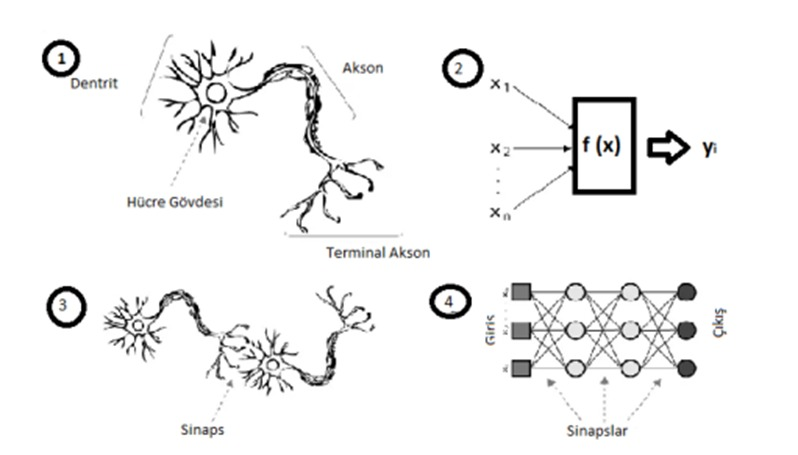
\includegraphics[width=1\linewidth,height=0.27\textheight]{figure/ysa_1} 

}

\caption{Biyolojik sinir hücresi ve yapay sinir ağı}\label{fig:ysa}
\end{figure}
(Maltarollo, Honório ve Silva, 2013)

Biyolojik sinir hücresi ve yapay sinir ağı benzetimleri \ref{fig:ysa}.'de verilmiştir.YSA, yapay sinir hücrelerinin birbirleri ile çeşitli şekillerde bağlanmasından oluşur ve genellikle katmanlar halinde düzenlenir.İnsan beynine iki şekilde benzerlik göstermektedir:
\begin{itemize}
\tightlist
\item
  Bilgi, öğrenme süreci yoluyla ağ tarafından elde edilir.
\item
  Sinaptik ağırlıklar olarak bilinen nöronlar arası bağlantı kuvvetlerini, bilgiyi depolamak için kullanır
\end{itemize}
\begin{figure}

{\centering 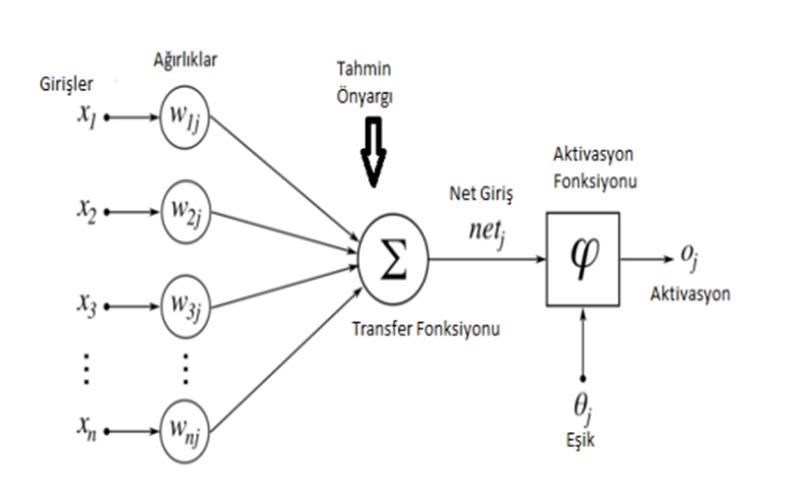
\includegraphics[width=1\linewidth,height=0.27\textheight]{figure/ysa_2} 

}

\caption{Yapay sinir hücresi}\label{fig:ysa2}
\end{figure}
(Öztürk ve Şahin, 2018)

\ref{fig:ysa2}. 'de görüldüğü gibi bir hücreye n adet veri girişi yapılmıştır.Bu girdilere ait ağırlıklar ile girilen veriler çarpılıp toplanması ile elde edilen transfer fonksiyonu, tranfer fonksiyonundan gelen değerin belirli bir aralığa normalize edildiği aktivasyon fonksiyonu ve aktivasyondan oluşur.
Çok katmanlı yapay sinir ağlarına bakıldığında temel olarak 3 katmandan meydana gelir;
\begin{itemize}
\tightlist
\item
  Girdi Katmanı (Input Layer)
\item
  Gizli, Ara Katmanlar (Hidden Layers)
\item
  Çıktı Katmanı (Output Layer)
\end{itemize}
Yapay Sinir Ağları uygulamaları en çok tahmin, sınıflandırma, veri ilişkilendirme, veri yorumlama ve veri filtreleme işlemlerinde kullanılmaktadır(Ağyar, 2015).

Bu prensipte çalışan yapay sinir ağları girdi değerinden çıktıları tahmin etme üzerine çalışır, örneğin altın ons fiyatının tahmini.

Bu doğrultuda kodlanan yapay ağlar toplanan veriler arasından en işe yarayan verileri kullanır.
\begin{itemize}
\tightlist
\item
  Sınıflandırma Girdi değerlerini sınıflandırarak sistemin daha hızlı sonuca varmasına etkide bulunur.
\end{itemize}
Önceden eğitilen ağ girdilerini analiz eder, bir olay hakkında bu girdiler sayesinde yeni yorumlamalar yapabilmektedir.

Öğrendiği bilgilerle konuları ilişkilendirir ve bunun sonucunda ortaya çıkan eksik bilgileri tamamlar(Öztürk ve Şahin, 2018).

Bir yapay sinir ağının yapısı ve sinir hücrelerinin sayısı değişiklik göstermelerine rağmen, yapay sinir ağının oluşumu için kabul görmüş herhangi bir kural bulunmamaktadır.Gerekli gizli katman sayısından az gizli katmana sahip yapay sinir ağları komplike fonksiyonların çözümünde yetersiz kalırken, çok fazla gizli katmana sahip yapay sinir ağları ise istenmeyen kararsızlıklarla karşılaşmaktadır.Gizli katman sayısı belirlendikten sonra karşılaşılan problem ise her bir tabakada kaç tane nöronun yer alacağına karar vermede karşımıza çıkmaktadır.Girdi katmanı için bir sorun bulunmamaktadır.Bu sayı sistem içerisindeki girdilerin sayısına eşittir.Aynı şekilde, çıktı katmanı da istenilen çıktı sayısıyla belirlenebilmektedir.Esas sorun, gizli katmanlarda nöron sayısını belirlemektir.Geleneksel matris algoritması, matris boyutlarının ya girdi sayısına ya da çıktı sayısına eşit olması gerektiğini söylemektedir.Ne yazık ki, gizli katmanda en verimli şekilde kaç tane nöronun bulunacağı konusunda herhangi bir matematiksel test bulunmamaktadır.Deneme ve yanılma yöntemi uygulanarak karar verilmelidir(Bell, Detienne ve Joshi, 2003).
\begin{figure}

{\centering 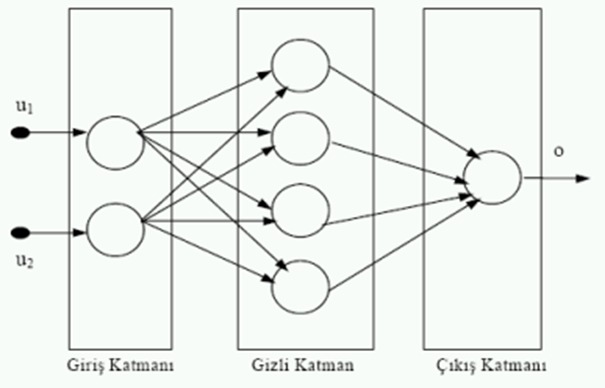
\includegraphics[width=1\linewidth,height=0.27\textheight]{figure/ysa_3} 

}

\caption{İleri beslemeli sinir ağı yapısı}\label{fig:ysa3}
\end{figure}
(Fırat ve Güngör, 2004)

YSA, hücrelerin bağlanma biçimlerine göre ``ileri beslemeli'' ve ``geri beslemeli'' olmak üzere iki mimari yapı altında sınıflandırılabilmektedir

\hypertarget{ileri-beslemeli-aux11flar}{%
\subsubsection{İleri beslemeli ağlar}\label{ileri-beslemeli-aux11flar}}

Verilerin sadece girdi birimlerinden çıktı birimlerine ileri doğru aktığı ağ yapısıdır.Bu yapıda nöronlar katmanlar şeklinde düzenlenir.Bir katmandaki nöronların çıkışları bir sonraki katmana ağırlıklar üzerinden giriş olarak verilir.Aynı katmandaki nöronlar arasında veya bir önceki katmana bağlantı yani geri besleme çevrimi yoktur.Uygulamalarda genellikle ileri beslemeli ağların tercih edildiği görülmektedir(Asilkan ve Irmak, 2009).

\hypertarget{geri-beslemeli-aux11flar}{%
\subsubsection{Geri beslemeli ağlar}\label{geri-beslemeli-aux11flar}}

Veri akışının sadece ileriye doğru değil geriye doğru da olabileceği ağ yapısıdır.Bu yapıda en az bir tane geri besleme çevirimi bulunur.Geri besleme, aynı katmandaki hücreler arasında olabileceği gibi farklı katmanlardaki nöronlar arasında da olabilir(Asilkan ve Irmak, 2009).

İşlem sürecinde toplama ve aktivasyon adlarında iki fonksiyon yer almaktadır.
Toplama (Birleştirme) Fonksiyonu: Yapay sinir hücresine gelen girdilerin kendilerine ait ağırlıklarla çarpıldıktan sonra birleştirilmesi işlemini gerçekleştiren fonksiyondur.Bu fonksiyon, adından da anlaşılacağı gibi, genelde toplama işlemini kullanmakla birlikte farklı işlemleri de kullanabilir.Hatta araştırmacının kendi kurduğu işlemi de kullanması mümkündür.Toplama fonksiyonunda kullanılan işlem, genellikle seçilen ağ mimarisine de bağlıdır.En sık kullanılan fonksiyonlar şunlardır; Toplama, çarpım, maksimum, minimum, çoğunluk, kümülatif toplamdır(Asilkan ve Irmak, 2009).

Yapay sinir hücresinin çıktısının büyüklüğünü sınırlandıran fonksiyondur.Bazı kaynaklarda transfer, eşik veya sıkıştırma fonksiyonu olarak da isimlendirilmektedir(Mandic ve Chambers, 2001).Bir ağdaki tüm hücrelerin aktivasyon fonksiyonu birbirinden farklı olabilir.Aktivasyon fonksiyonunda doğrusal fonksiyonlar genelde tercih edilmez.Zaman serileri için ``Sigmoid'', ikili (binary) değişkenler için ``Adım'' fonksiyonu önerilmektedir(Tebelskis, 1995).En çok kullanılan aktivasyon fonksiyonları şunlardır: Doğrusal, adım, eşik değer, hiperbolik tanjant, sigmoidtir(Asilkan ve Irmak, 2009).

Derin ağlar, görüntü tanıma, nesne tanıma ve doğal dil işleme gibi birçok alanda kullanılmaktadır.Aktivite tanıma alanında derin öğrenme yöntemleri ile son yıllarda çalışmalar yapılmıştır.Bu alanda derin öğrenme yöntemleri kullanmanın en büyük avantajı ham sensör verilerinden saklı kalmış önemli özelliklerin otomatik çıkartılabilmesidir.Aktivite tanıma için sensör verilerinden hangi özelliklerin kullanılacağını belirlemek için bilirkişiye ihtiyaç kalmamaktadır.Derin ağlarla cihaz konumundan ve oryantasyonundan bağımsız özellikler de çıkartılabilmektedir.

Derin ağların eğitim süresi çok uzun süreler alabildiği için süreyi kısaltmak adına güçlü donanımların kullanımına ihtiyaç duyulmaktadır.Dolayısıyla derin öğrenme ile eğitimin şu anki mobil cihaz donanımları üzerinde yapılması mümkün değildir.Sadece bilgisayar ortamında eğitilmiş hazır modeller telefon üzerinde gerçek zamanlı aktivite sınıflandırmak için kullanılabilir.
Derin öğrenme yöntemlerinin her birisinin farklı çalışma prensipleri vardır.İncelenmiş makaleler içerisinde daha çok tercih edilen ağ Konvolüsyonel Sinir Ağları (Convolutional Neural Network) olmuştur.Kullanılan derin öğrenme yöntemleri ve sonuçlar karşılaştırmalı(Iskanderov ve Güvensan, 2019).

\hypertarget{tekrarlayan-sinir-aux11flarux131-recurrent-neural-network}{%
\subsection{Tekrarlayan Sinir Ağları (Recurrent Neural Network)}\label{tekrarlayan-sinir-aux11flarux131-recurrent-neural-network}}

TSA, zaman serilerini kullanarak işlemleri gerçekleştiren bir YSA türüdür.İleri beslemeli ağların çalışma mantığından farklı olarak ağın girdi verileri TSA eğitimlerinde kullanılabilmektedir.Geri yayılım (backpropagation) ise YSA'lara benzer olarak gerçekleştirebilmektedir.TSA ağları, aynı yapıya sahip TSA hücrelerinin birbirinden farklı gizli durumlarını işleyen kopyalarının bir araya gelmesi ile oluşmaktadır.Bu kopyalar TSA hücrelerinin gizli olmasına neden olmaktadır.Bu derin mimari modelinin tekrarlayan olarak isimlendirilmesinin sebebi çıktı verilerinin tekrardan girdi verisi olarak kullanılmasıdır (Metin ve Karasulu, 2021a; Metın ve Karasulu, 2019).
\begin{figure}

{\centering 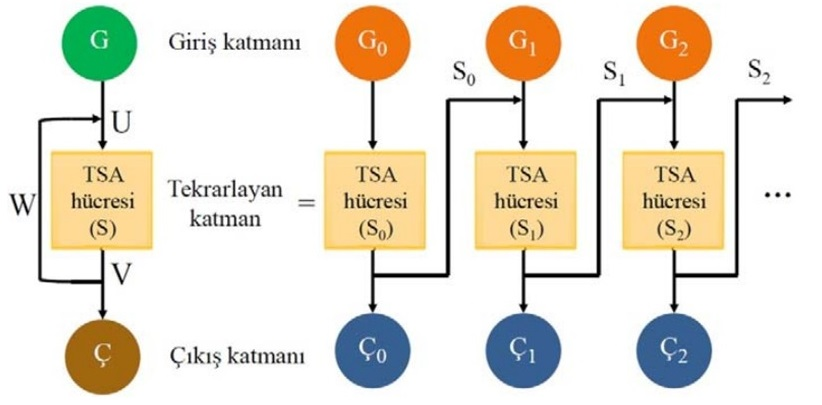
\includegraphics[width=1\linewidth,height=0.27\textheight]{figure/rnn_1} 

}

\caption{TSA‘nın genel yapısı}\label{fig:ysa4}
\end{figure}
\ref{fig:ysa4} 'de TSA'nın genel yapısı gösterilmektedir(Eşref, 2019).

Burada, St değeri ile TSA hücrelerinin t anındaki gizli durumları ifade edilmektedir.Bu yöntem yardımı ile o anki adıma kadar ağa giren tüm girdi verileri üzerinden buradaki t anında işleme alınan Gt durumundaki girdi verisi hesaplanmaktadır.Ayrıca, (t - 1) anındaki mevcut gizli durum ise St-1 değeriyle ifade edilmektedir.Aşağıdaki \(S_{t}\) eşitliğinde görülebileceği gibi uygun model oluşturularak buna ait U ve W ağırlık parametreleri kullanılmasıyla St değeri hesaplanmaktadır.

Bu eşitlikteki \(f_{a}\) aktivasyon fonksiyonunu ifade etmektedir.Genellikle burada hiperbolik tanjant (tanh) aktivasyon fonksiyonu seçilerek {[}-1,1{]} aralığında sonuç üretmektedir(Z. Yang, Salakhutdinov ve Cohen, 2016).

\[ S_{t} = f_{A}(UG_{t}+WS_{t-1})\]
belirtilen hesaplamada normalize işlemi gerçekleştirilmiş softmax fonksiyonu kullanılarak {[}0,1{]} değerleri arasında ağın çıktısı \({Ç_[t]}\) elde edilmektedir.

\[Ç_{t} = softmax(V * S_{t})\]

YSA`da girdi verileri tüm katmanlarda kullanıldığından gradyan değeri önceki katmanlara bağımlı biçimde değişmektedir.Geri yayılımın sürekli yenilenmesi sonrasında, hesaplamalardaki değerlerde azalma yaşanması sonucu kaybolan gradyan (vanishing gradient) problemi oluşabilmekte, buna benzer diğer bir durumdaysa 1'den büyük değer alan gradyanlar hesaplanan sonucun büyümesine yol açmaktadırlar.Bu durumda da patlayan gradyan (exploiting gradient) problemi ortaya çıkmaktadır.Oluşan bu problemlerin en aza indirilmesi için, uzun süreli bağımlılıkları da öğrenebilen yapıdaki TSA mimarisinin özel bir tipi olan UKSB hücreleri kullanılmaktadır.Uzun vadeli bağımlılık ve kaybolan gradyan gibi problemlere çözüm için geliştirilmiş olan ve TSA mimarisi göz önüne alındığında daha hızlı ve görece daha basit yapıda olan Kapılı Tekrarlayan Birim (KTB) modelleri de literatürde mevcuttur.Bu mimari bakış açısıyla, unutma kapısı (forget gate), girdi kapısı (input gate) ve çıktı kapıları (output gate) UKSB hücrelerinde bulunmaktadır(Z. Yang ve diğerleri, 2016).KTB hücreleri reset kapısı ve güncelleme kapısı (update gate) içermekte, böylece UKSB hücrelerine göre hafızada bir verinin ne kadar uzun süre tutulup, güncel veri ile hafızadaki verinin hangi zaman adımında birleştirileceği gibi olgular belirlenebilmektedir(Z. Yang ve diğerleri, 2016).Veri dizileri içerisinde belirli bir önceki (t - 1) ve buna ilişkin sonraki (t + 1) zaman adımlarını işleyebilen çift yönlü işlevsel yapılar da literatürdeki çeşitli çalışmalarda mevcuttur.Çift yönlü işlevsel bir yapıya sahip olarak oluşturulan KTB ve UKSB hücrelerini içeren çeşitli modellerin aynı zamanda ardışık verileri işlemede bazı avantajları da vardır (Schuster ve Paliwal, 1997).

\hypertarget{evriux15fimli-sinir-aux11flarux131-convolutional-neural-network}{%
\subsection{Evrişimli Sinir Ağları (Convolutional Neural Network)}\label{evriux15fimli-sinir-aux11flarux131-convolutional-neural-network}}

ESA, görme duyusunun işlevinden faydalanan, görüntüleri alt bölümlere parçalayarak bütün görüntü üzerinde işlem yapan Çok Katmanlı Algılayıcı (ÇKA) türüdür.1988 yılında Yann LeCun'ın öne sürdüğü ve 1998 yılına kadar da üzerinde iyileştirmelerin gerçekleştirildiği ilk ESA ağlarından birisi de LeNet ağıdır(Metin ve Karasulu, 2021b).LeNet ağında; ÇKA yapısına benzeyen tam bağlı katman (fully connected layer), biriktirme katmanı (pooling layer) ve evrişim katmanı (convolution layer) yer almaktadır(LeCun, Bottou, Bengio ve Haffner, 1998).ESA, veriyi işlerken çeşitli filtreler kullanmakta, bu filtrelerin içerikleri veriden elde edilen öznitelikler olarak otomatik bir biçimde ağ tarafından öğrenilebilmektedir.\ref{fig:cnn1}.'te ESA ağının iki boyutlu (2B) yapıda oluşturulan modeline dair altyapı şematik olarak görülmektedir(Bengio, Courville ve Vincent, 2013).ESA modellerinin katmanları incelendiğinde; evrişim katmanı ESA'nın temelini oluşturan dönüşüm katmanıdır.Bu katmanda, belirli ölçeklerdeki filtreler görüntüler üzerinde kaydırılarak öznitelik haritasının (feature map) oluşturulması sağlanır.Biriktirme katmanı; evrişim katmanları arasına eklenen katmandır.Model içerisinde parametre değerlerinin hesaplama miktarını azaltarak aşırı öğrenme (overfitting) nedeniyle ağ'da oluşan ezberlemeyi önler.Bu sayede ağ üzerinde uyumsuz durumların da engellenmesi sağlanmış olur. Düzleştirilmiş (flatten) veriler, tam bağlı katmanda alınarak sinir ağı vasıtasıyla öğrenme işlemi gerçekleştirilmektedir. İşlemler sonrasında belirlenen sınıflara göre dönüşümler gerçekleştirilmektedir.Bazı katmanlardaki sinir düğümlerinin eğitim süresi içerisinde pasif bir duruma getirilmesi ise iletim sönümü (dropout) katmanında gerçekleştirilir.Sadece ve sadece eğitim süresi içerisinde iletim sönümü gerçekleştirilmekte, tüm sinir düğümleriyse test işlemi süresince aktif durumda olmaktadır.
\begin{figure}

{\centering 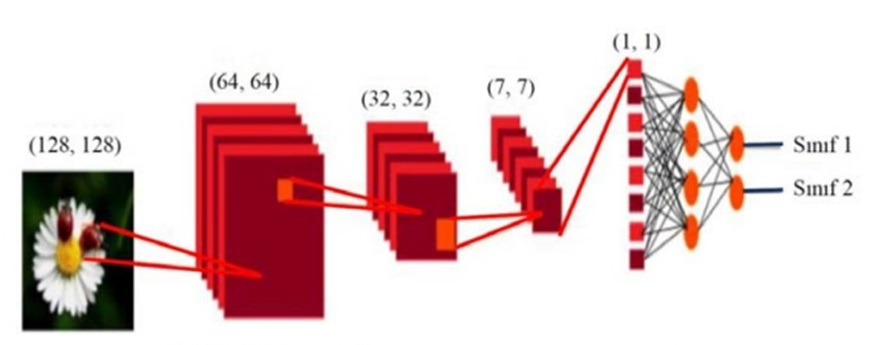
\includegraphics[width=1\linewidth,height=0.27\textheight]{figure/cnn_1} 

}

\caption{Evrişimli Sinir Ağları Yapısı}\label{fig:cnn1}
\end{figure}
(Metın ve Karasulu, 2019)

Böylece iletim sönümü kullanımıyla; çok fazla ayrıntıya ağ modelinin odaklanması da engellenerek başarım iyileştirilmektedir.Her bir döngü süresince belirli bir oranda farklı sinir düğümleri böylece pasif hale getirilmekte ve aktif haldeki sinir düğümleriyse sürekli değiştirilmektedir(LeCun ve diğerleri, 1998).Ara katmanların doğrusal olmayan biçimde veriyi işlemesinde aktivasyon fonksiyonu olarak doğrultulmuş biçimli doğrusal birim olarak bilinen ReLU (Rectified Linear Unit) içeren bir yapı sıklıkla literatürdeki çalışmalarda kullanılmaktadır(Buduma, 2017).Bu fonksiyon sayesinde öznitelikler üzerinde belirli bir filtreleme de yapılmaktadır.

Günümüzde çeşitli duyargalardan elde edilen sinyal verilerinin işlenmesine dayanan çalışmalar literatürde oldukça popüler bir araştırma alanı olmuştur.Özellikle bu tip sinyal verilerinden elde edilen öznitelikler literatürdeki ilgili çalışmalarda klasik makine öğrenmesi veya derin öğrenme teknikleri ile kullanılmakta, insan aktivitelerinin tespiti ve sınıflandırılması, bu aktiviteler sayesinde cinsiyet belirleme gibi çeşitli konulardaki birçok problemin çözümü adına uygulamaya yönelik çalışmalar yapılmaktadır(Kuncan ve Kaya, 2019).Derin öğrenme ağ mimari modelleri gerçek hayattaki problemlere çözüm üreten birçok çalışmada sıklıkla kullanılmaktadır.Özellikle ham veriden otomatik olarak öznitelik öğrenebilme yeteneği ve yüksek doğruluktaki başarımı sayesinde derin öğrenme modelleri gün geçtikçe çalışmalarda daha çok tercih edilir olmaktadır.Derin öğrenme için belli başlı ağ mimari modelleri çeşitli araştırma alanlarındaki çalışmalarda kullanılmaktadır.Literatürdeki örnek teşkil eden son yıllardaki güncel bazı çalışmalara baktığımızda; görüntü işleme tabanlı olarak köpeklerin davranışlarının incelenmesiyle bunlara dair verilerin daha hızlı bölgesel ESA ağ modeli ile sınıflandırılmasında (Dandıl ve Polattimur, 2020), uydu duyargaları ile elde edilen hiperspektral görüntülerin ESA ağ modeli ile sınıflandırılmasında (Hanbay, 2020) ve ses sinyallerinin işlenmesi tabanlı olarak UKSB ağ modelinin kullanıldığı prozodik açıdan Türkçe ağız tanımada (Isık ve Artuner, 2020) derin öğrenme sayesinde yüksek doğrulukta başarım elde edildiği görülmektedir.Bu bakış açısıyla çalışmamızda duyarga sinyallerinden elde edilen öznitelikler kullanılarak derin öğrenme ağ mimari modelleriyle sınıflandırma yapılmasına dayanan uygulamaya yönelik bir çalışma yapılmıştır.

\hypertarget{makine-uxf6ux11frenmesi-deux11ferlendirme-uxf6luxe7uxfctleri}{%
\section{Makine öğrenmesi değerlendirme ölçütleri}\label{makine-uxf6ux11frenmesi-deux11ferlendirme-uxf6luxe7uxfctleri}}

Veriler kullanılarak, birçok farklı makine öğrenmesi algoritması ile farklı modeller oluşturmak mümkündür. Oluşturulan modellerden hangisinin daha iyi sonuç vereceğini ölçmek için değerlendirme metriklerine ihtiyaç duyulmaktadır. Değerlendirme metrikleri modelden elde edilen tahminler ile gerçek sonuçları karşılaştırarak bize rakamsal sonuçlar vermektedirler. Makine öğrenmesi modellerinin doğruluğu, 4 farklı değerlendirme metriği ile ölçülür.Karışıklık matrisi, sınıflandırma yapan uygulamalarda, gerçek ve tahmin edilen değerleri bir tablo üzerinden kolayca kıyaslayabilmek için kullanılmaktadır(Kelle ve Hüseyin, 2022).
\begin{figure}

{\centering 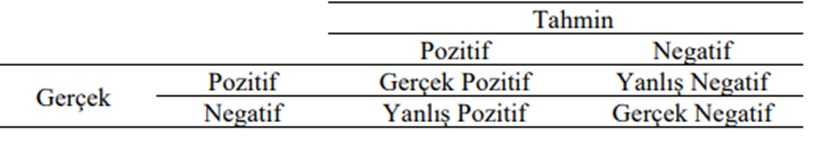
\includegraphics[width=0.7\linewidth,height=0.2\textheight]{figure/conf_mat} 

}

\caption{Karışıklık matrisi örneği}\label{fig:confmat}
\end{figure}
(Kelle ve Hüseyin, 2022)

\ref{fig:confmat}.'de yer alan matriste;
\begin{itemize}
\tightlist
\item
  Gerçek Pozitif (GP): Doğru olarak tahmin edilen, gerçekte de doğru olan değerler,
\item
  Gerçek Negatif (GN): Yanlış olarak tahmin edilen, gerçekte de yanlış olan değerler,
\item
  Yanlış Pozitif (YP): Doğru olarak tahmin edilen, gerçekte yanlış olan değerler,
\item
  Yanlış Negatif (YN): Yanlış olarak tahmin edilen, gerçekte doğru olan değerleri ifade etmektedir.
\end{itemize}
\hypertarget{doux11fruluk-accuracy}{%
\subsubsection{Doğruluk (Accuracy)}\label{doux11fruluk-accuracy}}

Doğru tahmin edilen değerlerin, tüm değerlere bölünmesi ile elde edilmektedir. Doğruluk değeri, 0 ile 1 arasındadır. Doğruluk değeri 1'e yaklaştıkça başarı artmaktadır(Kelle ve Hüseyin, 2022).

\[Doğruluk = \frac{(GP + GN)}{(GP + GN + FP + FN)}\]

\hypertarget{duyarlux131lux131k-recall}{%
\subsubsection{Duyarlılık (Recall)}\label{duyarlux131lux131k-recall}}

Doğru olarak tahmin etmemiz gereken değerlerin, ne kadarını doğru tahmin ettiğimizi belirtmektedir. Duyarlılık değeri, gerçekte doğru olan ve doğru olarak tahmin edilen değerlerin, tüm doğru değerlere bölünmesi ile elde edilmektedir(Kelle ve Hüseyin, 2022).

\[Duyarlilik =  \frac{GP}{(GP + FN)}\]

\hypertarget{kesinlik-precision}{%
\subsubsection{Kesinlik (Precision)}\label{kesinlik-precision}}

Doğru olarak tahmin ettiğimiz değerlerin, ne kadarının gerçekte doğru olduğunu göstermektedir. Kesinlik değeri, gerçekte doğru olan ve doğru olarak tahmin edilen değerlerin, doğru olarak tahmin edilen tüm değerlere bölünmesi ile elde edilmektedir(Kelle ve Hüseyin, 2022).

\[Kesinlik =  \frac{GP}{(GP + FP)}\]

\hypertarget{f1-skoru-f1-score}{%
\subsubsection{F1 Skoru (F1 Score)}\label{f1-skoru-f1-score}}

F1 skoru, duyarlılık ve kesinlik değerlerinin harmonik ortalamasının hesaplanması ile elde edilmektedir. Her iki değerinde hesaplamaya katılarak dengeli bir değer elde edilmesi amaçlanmaktadır. Eşit dağılıma sahip olmayan veri setlerinde başarılı sonuçlar elde etmek için kullanılmaktadır(Kelle ve Hüseyin, 2022).

\[ F1 Skoru = \frac{2 * Kesinlik * Duyarlılık}{(Kesinlik + Duyarlılık)} \]

\hypertarget{ref-labels}{%
\chapter{UYGULAMA}\label{ref-labels}}

\hypertarget{uygulama}{%
\section{Uygulama}\label{uygulama}}

Bu bölümde akıllı telefon sensörleri ile elde edilen insan aktivitesi tanıma verileri kullanılmıştır(Anguita ve diğerleri, 2013). Gözlemler, jiroskop ve ivmeölçer sensörlerinden 100hz frekans, 1.28 saniyelik pencere aralığı ile elde edilmiştir.
Sınıflandırma yöntemleri olarak K En Yakın Komşular, Rassal Ormanlar, XGBoost, Destek Vektör Makinesi, Yapay Sinir Ağları yöntemleri kullanılmıştır.Takip eden bölümde uygulamada kullanılan veriler tanıtılmış ve keşifsel veri analizi sonuçlarına yer verilmiştir.
Kullanılan verilerde, Jiroskop ve ivmeölçerden elde edilen X,Y,Z eksenlerindeki ölçümler üzerinde aşağıdaki istatistiksel fonksiyonlar kullanılarak 561 değişken türetilmiştir.Veriler -1,1 aralığında olacak şekilde normalize edilmiştir.
\begin{itemize}
\tightlist
\item
  mean(): Ortalama
\item
  std(): Standart sapma
\item
  mad(): Medyan mutlak sapma
\item
  max(): Dizideki en büyük değer
\item
  min(): Dizideki en küçük değer
\item
  sma(): Sinyal büyüklük alanı
\item
  energy(): Karelerin toplamı bölü değer sayısı (enerji ölçüsü)
\item
  iqr(): Çeyrekler arası aralık
\item
  entropy(): Sinyal entropisi
\item
  arCoeff(): Burg mertebesi 4'e eşit olan otoregresyon katsayıları
\item
  correlation(): İki sinyal arasındaki korelasyon katsayısı
\item
  maxInds(): En büyük genliğe sahip frekans bileşeninin indeksi
\item
  meanFreq(): Ortalama bir frekans elde etmek için frekans bileşenlerinin ağırlıklı ortalaması
\item
  skewness(): Frekans alanı sinyalinin çarpıklığı
\item
  kurtosis(): Frekans alanı sinyalinin basıklığı
\item
  bandsEnergy(): Her pencerenin FFT'sinin 64 kutusu içindeki bir frekans aralığının enerjisi
\item
  angle(): Vektör arasındaki açı
\end{itemize}
\begin{figure}

{\centering 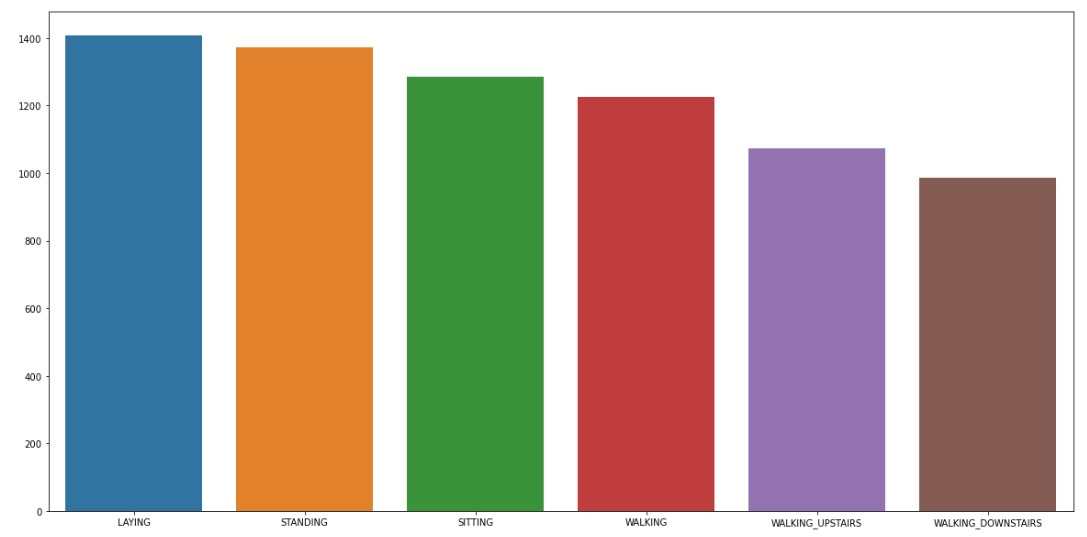
\includegraphics[width=1\linewidth,height=0.45\textheight]{figure/sınıf dağılımı} 

}

\caption{Hedef değişkene göre gözlem sayıları}\label{fig:freq}
\end{figure}
Hedef değişken; Yatma(0), Ayakta Durma (1), Oturma(2), Yürüme(3), Merdiven Çıkma(4), Merdiven İnme(5) olmak üzere 6 farklı kategoriye sahiptir. \ref{fig:freq}.' de hedef değişkene göre gözlem sayıları görselleştirilmiştir.
\begin{figure}
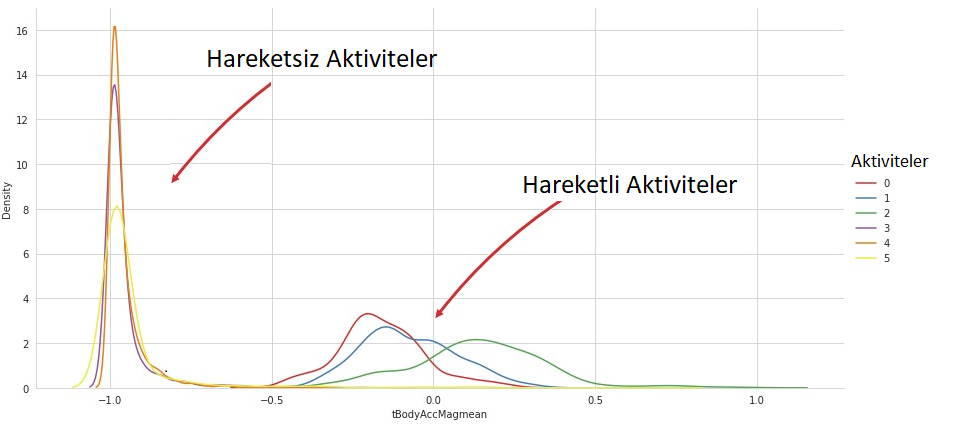
\includegraphics[width=1\linewidth,height=0.45\textheight]{figure/tbodyaccmagplot2} \caption{Sabit ve hareketli aktiviteler için tBodyAccMagmean değişkeninin yoğunluk grafiği}\label{fig:tbodyaccmagplot}
\end{figure}
\ref{fig:tbodyaccmagplot}. Veri setindeki `tBodyAccMagmean' değişkeninin yoğunluk grafiğidir.Aktiviteler, farklı renklerde gösterilmiş.Grafiğin sol tarafında ``Sabit Aktiviteler'' olarak adlandırılan Uzanma, Ayakta durma, Oturma, sağ tarafındaki ise ``Hareketli Aktiviteler'' olarak adlandırılan Yürüme, Merdiven inme, Merdiven çıkma aktivitelerini temsil etmektedir.
\begin{figure}
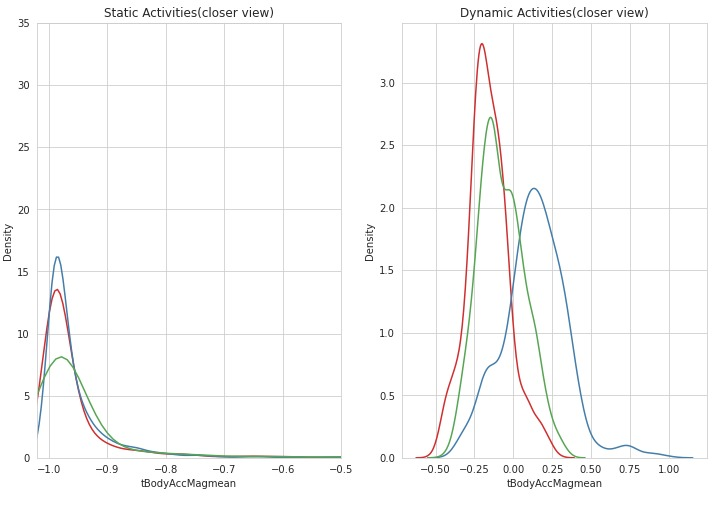
\includegraphics[width=1\linewidth,height=0.45\textheight]{figure/tbodyaccmag plot} \caption{Sabit ve hareketli aktivitelerin yoğunluk grafiklerinin karşılaştırılması}\label{fig:tbodyaccmagplot2}
\end{figure}
\ref{fig:tbodyaccmagplot2}. `tBodyAccMagmean' değişkeninin aktivitelere göre ayrılmış ve yakınlaştırılmış yoğunluk grafikleridir. İlk grafik, ``Oturma'', ``Ayakta durma'' ve ``Yatma'' aktivitelerini içerir ve yatay eksen, ``-1.02'' ile ``-0.5'' arasında bir aralığı kapsar.İkinci grafik ise ``Yürüme'', ``Aşağı inme'' ve ``Yukarı çıkma'' aktivitelerini içerir ve yine yatay eksen aynı aralıkta kısıtlanmıştır.Her iki grafik de, aktivitelerin ayrı ayrı dağılımlarını farklı renklerle gösterir ve dağılımların şekli hakkında bilgi sağlar.Bu grafiği oluşturmak için seaborn kütüphanesi kullanılmıştır.
\begin{figure}
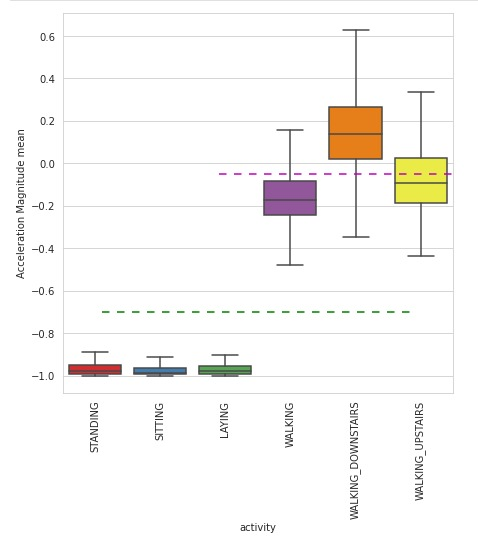
\includegraphics[width=1\linewidth,height=0.45\textheight]{figure/boxplot} \caption{tBodyAccMagmean Değişkeninin Aktivitilere Göre BoxPlot Grafiği}\label{fig:boxplot}
\end{figure}
\ref{fig:boxplot}. Her bir aktivitenin ortalama ivme büyüklüğünün dağılımını gösterir. Kesik çizgiler, değişkenin değerinin belirli bir eşiğin altında veya üstünde olma durumlarını gösterir. `y=- 0.7' çizgisi, sabit haldeki aktiviteler için eşiği temsil ederken, `y=- 0.05' çizgisi, hareket halindeki aktiviteler için eşiği temsil eder. Plt.axhline() fonksiyonu içerisindeki `dashes' parametresi, çizgilerin kesikli görüntüsünü sağlar. Bu grafiği oluşturmak için seaborn kütüphanesindeki fonksiyonlar kullanılmıştır. Aşağıdaki kurallar verideki tBodyAccMagmean değişkeninin aldığı değerlere göre aktivitelerin gruplanmasını göstermektedir;
\begin{itemize}
\tightlist
\item
  Eğer -0.8 \textgreater{} tBodyAccMagmean \textgreater{} -1 ise , sabit aktivite (ayakta, oturuyor veya uzanıyor) olarak değerlendirilebilir.
\item
  Eğer -0.6 \textless{} tBodyAccMagmean \textless{} 0.7 ise, hareketli aktivite (yürüyor, merdivenlerden aşağı iniyor ya da merdivenlerden yukarı çıkıyor) olarak değerlendirilebilir.
\end{itemize}
Araştırma çok sınıflı sınıflama problemi olarak ele alındığında makine öğrenmesi yöntemleri ile sınıflandırma modelleri geliştirilmesi gereklidir.

\hypertarget{uxe7ok-sux131nux131flux131-multiclass-sux131nux131flama-problemi}{%
\section{Çok Sınıflı (Multiclass) Sınıflama Problemi}\label{uxe7ok-sux131nux131flux131-multiclass-sux131nux131flama-problemi}}

Bu çalışmada akıllı telefon sensörleri ile elde edilen insan aktivitelerinin sınıflandırması Rassal Ormanlar , XGBoost, Destek Vektör Makinesi (SVM), K-En Yakın Komşuluk Modeli (KNN), Yapay Sinir Ağları yöntemleri kullanılmıştır. İlk olarak orijinal verilerdeki altı aktivite (Yürüme, Yukarı çıkma, Aşağı inme, Oturma, Ayakta, Yatma) için sınıflandırma hedeflenmiştir. Bölüm 3.1'de bu problem için farklı modeller ile elde edilen sonuçlara yer verilmiştir. Uygulamada Python programlama dili kullanılmış ve Scikit-Learn (Buitinck ve diğerleri, 2013), Pandas, Numpy, Matplotlib,LazyClassifier, SVM, XGBoost, KNeighborsClassifier Tensorflow, Keras kütüphanelerinden yararlanılmıştır.Modellerin performanslarını değerlendirmek üzere kesinlik, duyarlılık, F1-skoru, doğruluk oranı, dengelenmiş doğruluk oranı hesaplanmıştır.

Üç ayrı değişken grubu kullanılarak modellemeler yapılmıştır:
\begin{itemize}
\tightlist
\item
  Jiroskop Sensörüne Ait Değişkenler İle Modelleme
\item
  İvme Ölçer Sensörüne Ait Değişkenler İle Modelleme
\item
  Jiroskop ve İvme Ölçer Sensörlerine Ait Değişkenler İle Modelleme
\end{itemize}
Sensörlerin ayrı ayrı ve birlikte kullanılmasının modellerin performansına etkisi araştırılmıştır.
\begin{longtable}[]{@{}ll@{}}
\caption{\label{tab:nvar} Jiroskop ve İvme Ölçer Sensörlerinden elde edilen değişkenler}\tabularnewline
\toprule()
Değişkenler & Elde edilen değişken sayısı \\
\midrule()
\endfirsthead
\toprule()
Değişkenler & Elde edilen değişken sayısı \\
\midrule()
\endhead
fBodyGyro & 79 \\
fBodyAcc & 79 \\
fBodyAccJerk & 79 \\
tBodyAcc & 40 \\
tBodyAccJerk & 40 \\
tBodyGyro & 40 \\
tBodyGyroJerk & 40 \\
tGravityAcc & 40 \\
fBodyGyroJerkMag & 13 \\
fBodyGyroMag & 13 \\
fBodyAccJerkMag & 13 \\
fBodyAccMag & 13 \\
tBodyGyroJerkMag & 13 \\
tBodyGyroMag & 13 \\
tBodyAccJerkMag & 13 \\
tGravityAccMag & 13 \\
tBodyAccMag & 13 \\
angle & 7 \\
\bottomrule()
\end{longtable}
\begin{longtable}[]{@{}ll@{}}
\caption{\label{tab:nvargyro} Sadece Jiroskop Sensöründen elde edilen Değişkenler}\tabularnewline
\toprule()
Değişkenler & Elde edilen değişken sayısı \\
\midrule()
\endfirsthead
\toprule()
Değişkenler & Elde edilen değişken sayısı \\
\midrule()
\endhead
fBodyGryo & 79 \\
tBodyGyro & 40 \\
tBodyGyroJerk & 40 \\
tBodyGyroMag & 13 \\
tBodyGyroJerkMag & 13 \\
fBodyGyroMag & 13 \\
fBodyGyroJerkMag & 13 \\
angle & 5 \\
\bottomrule()
\end{longtable}
\begin{longtable}[]{@{}ll@{}}
\caption{\label{tab:nvaracc} Sadece İvmeölçer Sensöründen elde edilen Değişkenler}\tabularnewline
\toprule()
Değişkenler & Elde edilen değişken sayısı \\
\midrule()
\endfirsthead
\toprule()
Değişkenler & Elde edilen değişken sayısı \\
\midrule()
\endhead
fBodyAcc & 79 \\
fBodyAccJerk & 79 \\
tBodyAcc & 40 \\
tGravityAcc & 40 \\
tBodyAccJerk & 40 \\
tBodyAccMag & 13 \\
tGravityAccMag & 13 \\
tBodyAccJerkMag & 13 \\
fBodyAccMag & 13 \\
fBodyAccJerkMag & 13 \\
angle & 5 \\
\bottomrule()
\end{longtable}
\hypertarget{jiroskop-sensuxf6ruxfcne-ait-deux11fiux15fkenler-ile-modelleme}{%
\section{Jiroskop Sensörüne Ait Değişkenler İle Modelleme}\label{jiroskop-sensuxf6ruxfcne-ait-deux11fiux15fkenler-ile-modelleme}}

\hypertarget{knn-modeli}{%
\subsection{KNN Modeli}\label{knn-modeli}}

Bu bölümde jiroskop sensöründen elde edilen veriler kullanılmıştır.K-En yakın komşuluk modeli kurulmuş ve çıktıları değerlendirilmiştir.
\ref{tab:nvargyro}.' te belirtilen değişkenler kullanılarak modelleme gerçekleştirilmiştir.

\hypertarget{hiper-parametre-seuxe7imi}{%
\subsubsection{Hiper Parametre Seçimi}\label{hiper-parametre-seuxe7imi}}

Daha önce belirlenen parametre uzayını ve Scikit-Learn kütüphanesinde bulunan GridSearchCV algoritması ile en yüksek doğruluk oranı yakalanana kadar çalışması sağlanmıştır.
K-En yakın komşuluk modeli için en yüksek doğruluk oranı aşağıdaki parametreler ile bulunmuştur;
\begin{itemize}
\tightlist
\item
  `metric': `manhattan'
\item
  `n\_neighbors': 9
\item
  `weights': `distance'
\end{itemize}
\hypertarget{en-iyi-model}{%
\subsubsection{En İyi Model}\label{en-iyi-model}}

Bulunan parametrelerle kurulan modelin sınıflandırma metrikleri aşağıdaki gibidir.
\begin{longtable}[]{@{}lllll@{}}
\caption{\label{tab:jknn} Jiroskop Sensöründen elde edilen değişkenler ile kurulan k en yakın komşular modelinin başarı sonuçları}\tabularnewline
\toprule()
& precision & recall & F1-score & support \\
\midrule()
\endfirsthead
\toprule()
& precision & recall & F1-score & support \\
\midrule()
\endhead
0 & 0.70 & 0.84 & 0.77 & 496 \\
1 & 0.86 & 0.75 & 0.80 & 471 \\
2 & 0.76 & 0.71 & 0.74 & 420 \\
3 & 0.82 & 0.75 & 0.78 & 491 \\
4 & 0.79 & 0.89 & 0.84 & 531 \\
5 & 1.00 & 0.95 & 0.97 & 537 \\
Accuracy & & & 0.82 & 2946 \\
macro avg & 0.82 & 0.81 & 0.82 & 2946 \\
weighted avg & 0.83 & 0.82 & 0.82 & 2946 \\
\bottomrule()
\end{longtable}
\begin{figure}

{\centering 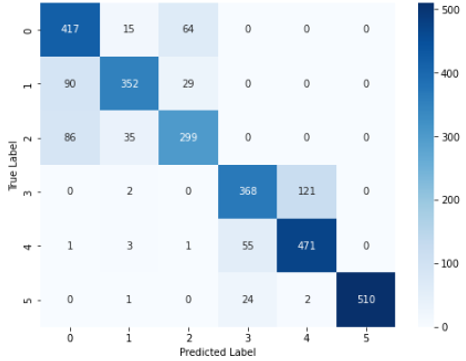
\includegraphics[width=0.9\linewidth,height=0.35\textheight]{figure/knn_conf} 

}

\caption{K-NN Modeli Karmaşıklık Matrisi}\label{fig:knnconf}
\end{figure}
\begin{figure}

{\centering 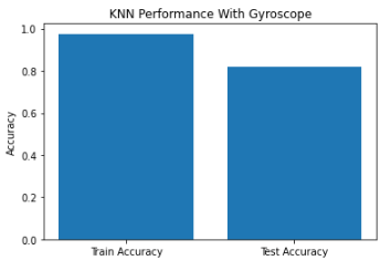
\includegraphics[width=0.6\linewidth,height=0.25\textheight]{figure/knn_testtrainaccuracy} 

}

\caption{K-NN Modelinin Eğitim ve Test Verilerinin Başarı Performansları}\label{fig:knntesttrain}
\end{figure}
\hypertarget{rassal-ormanlar-modeli}{%
\subsection{Rassal Ormanlar Modeli}\label{rassal-ormanlar-modeli}}

Bu bölümde jiroskop sensöründen elde edilen veriler kullanılmıştır.Rassal ormanlar modeli kurulmuş ve çıktıları değerlendirilmiştir.
\ref{tab:nvargyro}.' te belirtilen değişkenler kullanılarak modelleme işlemi gerçekleştirilmiştir.

\hypertarget{hiper-parametre-seuxe7imi-1}{%
\subsubsection{Hiper Parametre Seçimi}\label{hiper-parametre-seuxe7imi-1}}

Daha önce belirlenen parametre uzayını ve Scikit-Learn kütüphanesinde bulunan GridSearchCV algoritması ile en yüksek doğruluk oranı yakalanana kadar çalışması sağlanmıştır.
\begin{itemize}
\tightlist
\item
  max\_depth: 20
\item
  min\_samples\_leaf: 4
\item
  min\_samples\_split: 10
\item
  n\_estimators: 500
\end{itemize}
\hypertarget{en-iyi-model-1}{%
\subsubsection{En İyi Model}\label{en-iyi-model-1}}

Bulunan parametrelerle kurulan modelin sınıflandırma metrikleri aşağıdaki gibidir.
\begin{longtable}[]{@{}lllll@{}}
\caption{\label{tab:jrf} Jiroskop Sensöründen elde edilen değişkenler ile kurulan rassal ormanlar modelinin başarı sonuçları}\tabularnewline
\toprule()
& precision & recall & F1-score & support \\
\midrule()
\endfirsthead
\toprule()
& precision & recall & F1-score & support \\
\midrule()
\endhead
0 & 0.89 & 0.85 & 0.87 & 496 \\
1 & 0.89 & 0.94 & 0.92 & 471 \\
2 & 0.81 & 0.81 & 0.81 & 420 \\
3 & 0.97 & 0.88 & 0.92 & 491 \\
4 & 0.90 & 0.97 & 0.93 & 531 \\
5 & 1.00 & 1.00 & 1.00 & 537 \\
Accuracy & & & 0.91 & 2946 \\
macro avg & 0.91 & 0.81 & 0.91 & 2946 \\
weighted avg & 0.91 & 0.82 & 0.91 & 2946 \\
\bottomrule()
\end{longtable}
\begin{figure}

{\centering 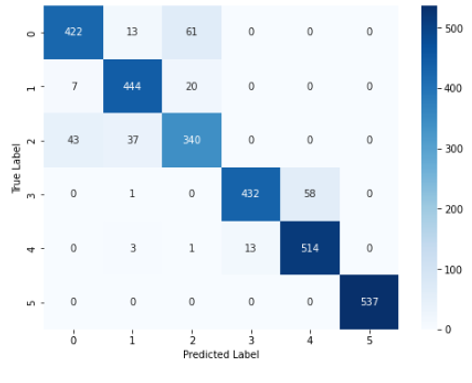
\includegraphics[width=0.9\linewidth,height=0.35\textheight]{figure/random_forest_confmat} 

}

\caption{Rassal Ormanlar Modeli Karmaşıklık Matrisi}\label{fig:randomforestconfmat}
\end{figure}
\begin{figure}

{\centering 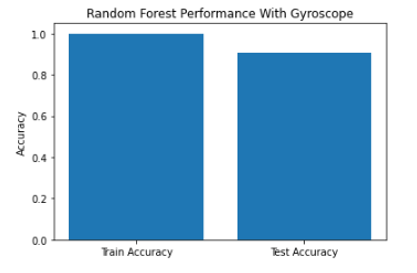
\includegraphics[width=0.6\linewidth,height=0.25\textheight]{figure/random_forest_testtrainaccuracy} 

}

\caption{Rassal Ormanlar Modelinin Eğitim ve Test Verilerinin Başarı Performansları}\label{fig:randomforesttesttrain}
\end{figure}
\newpage

\hypertarget{extreme-gradient-boosting-xgboost}{%
\subsection{eXtreme Gradient Boosting (XGBoost)}\label{extreme-gradient-boosting-xgboost}}

Bu bölümde jiroskop sensöründen elde edilen veriler kullanılmıştır.XGBoost modeli kurulmuş ve çıktıları değerlendirilmiştir.
\ref{tab:nvargyro}.' te belirtilen değişkenler kullanılarak modelleme işlemi gerçekleştirilmiştir.

\hypertarget{hiper-parametre-seuxe7imi-2}{%
\subsubsection{Hiper Parametre Seçimi}\label{hiper-parametre-seuxe7imi-2}}

Daha önce belirlenen parametre uzayını ve Scikit-Learn kütüphanesinde bulunan GridSearchCV algoritması ile en yüksek doğruluk oranı yakalanana kadar çalışması sağlanmıştır.
\begin{itemize}
\tightlist
\item
  max\_depth: 3
\item
  learning\_rate: 0.01
\item
  n\_estimators: 100
\end{itemize}
\hypertarget{en-iyi-model-2}{%
\subsubsection{En İyi Model}\label{en-iyi-model-2}}

Bulunan parametrelerle kurulan modelin sınıflandırma metrikleri aşağıdaki gibidir.
\begin{longtable}[]{@{}lllll@{}}
\caption{\label{tab:jxgboost} Jiroskop Sensöründen elde edilen değişkenler ile kurulan xgboost modelinin başarı sonuçları}\tabularnewline
\toprule()
& precision & recall & F1-score & support \\
\midrule()
\endfirsthead
\toprule()
& precision & recall & F1-score & support \\
\midrule()
\endhead
0 & 0.91 & 0.84 & 0.87 & 496 \\
1 & 0.84 & 0.90 & 0.87 & 471 \\
2 & 0.81 & 0.83 & 0.82 & 420 \\
3 & 0.94 & 0.86 & 0.90 & 491 \\
4 & 0.88 & 0.94 & 0.91 & 531 \\
5 & 1.00 & 1.00 & 1.00 & 537 \\
Accuracy & & & 0.90 & 2946 \\
macro avg & 0.90 & 0.89 & 0.89 & 2946 \\
weighted avg & 0.90 & 0.90 & 0.90 & 2946 \\
\bottomrule()
\end{longtable}
\begin{figure}

{\centering 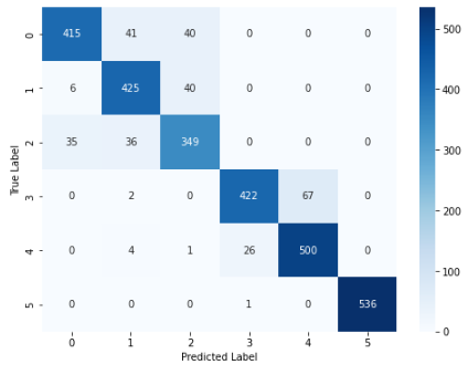
\includegraphics[width=0.9\linewidth,height=0.35\textheight]{figure/xgboost_confmat} 

}

\caption{XGBoost Modeli Karmaşıklık Matrisi}\label{fig:xgboostconfmat}
\end{figure}
\begin{figure}

{\centering 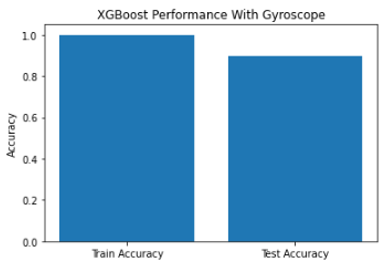
\includegraphics[width=0.6\linewidth,height=0.25\textheight]{figure/xgboost_testtrain} 

}

\caption{XGBoost Modelinin Eğitim ve Test Verilerinin Başarı Performansları}\label{fig:xgboosttesttrain}
\end{figure}
\hypertarget{destek-vektuxf6r-makinesi-1}{%
\subsection{Destek Vektör Makinesi}\label{destek-vektuxf6r-makinesi-1}}

Bu bölümde jiroskop sensöründen elde edilen veriler kullanılmıştır.Destek Vektör Makinesi (SVM) modeli kurulmuş ve çıktıları değerlendirilmiştir
\ref{tab:nvargyro}.' te belirtilen değişkenler kullanılarak modelleme işlemi gerçekleştirilmiştir.

\hypertarget{hiper-parametre-seuxe7imi-3}{%
\subsubsection{Hiper Parametre Seçimi}\label{hiper-parametre-seuxe7imi-3}}

Daha önce belirlenen parametre uzayını ve Scikit-Learn kütüphanesinde bulunan GridSearchCV algoritması ile en yüksek doğruluk oranı yakalanana kadar çalışması sağlanmıştır.
\begin{itemize}
\tightlist
\item
  C: 0.1
\item
  gamma: 0.01
\item
  kernel: linear
\end{itemize}
\hypertarget{en-iyi-model-3}{%
\subsubsection{En İyi Model}\label{en-iyi-model-3}}

Bulunan parametrelerle kurulan modelin sınıflandırma metrikleri aşağıdaki gibidir.
\begin{longtable}[]{@{}lllll@{}}
\caption{\label{tab:jsvm} Jiroskop Sensöründen elde edilen değişkenler ile kurulan destek vektör makinası modelinin başarı sonuçları}\tabularnewline
\toprule()
& precision & recall & F1-score & support \\
\midrule()
\endfirsthead
\toprule()
& precision & recall & F1-score & support \\
\midrule()
\endhead
0 & 0.86 & 0.89 & 0.88 & 496 \\
1 & 0.94 & 0.94 & 0.94 & 471 \\
2 & 0.83 & 0.83 & 0.83 & 420 \\
3 & 0.92 & 0.88 & 0.90 & 491 \\
4 & 0.90 & 0.92 & 0.91 & 531 \\
5 & 1.00 & 1.00 & 1.00 & 537 \\
Accuracy & & & 0.91 & 2946 \\
macro avg & 0.91 & 0.91 & 0.91 & 2946 \\
weighted avg & 0.91 & 0.91 & 0.91 & 2946 \\
\bottomrule()
\end{longtable}
\begin{figure}

{\centering 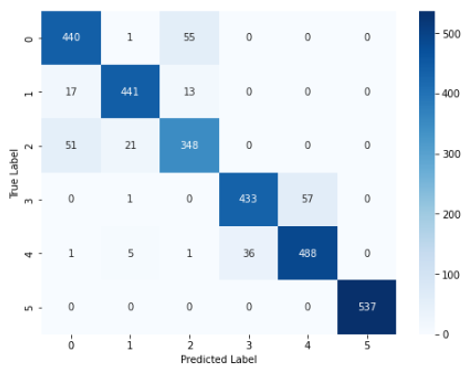
\includegraphics[width=0.9\linewidth,height=0.35\textheight]{figure/svm_confmat} 

}

\caption{Destek Vektör Makinesi Modeli Karmaşıklık Matrisi}\label{fig:svmconfmat}
\end{figure}
\begin{figure}

{\centering 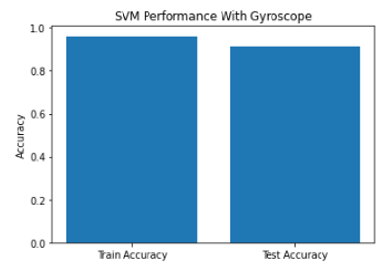
\includegraphics[width=0.6\linewidth,height=0.25\textheight]{figure/svm_testtrain} 

}

\caption{Destek Vektör Modelinin Eğitim ve Test Verilerinin Başarı Performansları}\label{fig:svmtesttrain}
\end{figure}
\hypertarget{yapay-sinir-aux11flarux131-neural-networks}{%
\subsection{Yapay Sinir Ağları (Neural Networks)}\label{yapay-sinir-aux11flarux131-neural-networks}}

Bu bölümde jiroskop sensörü üzerinde yapay sinir ağları modeli kullanılmış ve çıktıları değerlendirilmiştir.Tensorflow ve Keras kütüphanelerindeki Sequential() fonksiyonu kullanılmıştır.

\hypertarget{kullanux131lan-katmanlar}{%
\subsubsection{Kullanılan Katmanlar}\label{kullanux131lan-katmanlar}}

İlk katman, tamamen bağlı (Dense) katmandır. Bu katman 64 nörona sahiptir ve girdi boyutu, train veri kümesinin özellik sayısına eşittir. kernel\_initializer parametresi ``normal'' olarak ayarlanmıştır, yani rastgele normal bir dağılım kullanılarak başlangıç ağırlıkları oluşturulacaktır. Bu katmanın aktivasyon fonksiyonu ``sigmoid'' olarak ayarlanmıştır.
İkinci katman, bir Dropout katmanıdır. Dropout, ağdaki aşırı uyumu azaltmak için kullanılan bir düzenleme tekniğidir. Bu katmanın Dropout oranı \%20 olarak ayarlanmıştır.
Üçüncü ve son katman, yine bir tamamen bağlı (Dense) katmandır. Bu katman 6 nörona sahiptir ve softmax aktivasyon fonksiyonu kullanılarak çoklu sınıflandırma işlemi gerçekleştirilir. kernel\_initializer parametresi ``normal'' olarak ayarlanmıştır.
Modelin derlenmesi, ``adam'' optimizasyon algoritması kullanılarak gerçekleştirilir. Kayıp fonksiyonu ``sparse\_categorical\_crossentropy'' olarak ayarlanmıştır, çünkü etiketler doğrudan kategorik olarak kodlanmamıştır. Ölçülen metrik, doğruluk (accuracy) olarak ayarlanmıştır.
\ref{tab:nvargyro}.' te belirtilen değişkenler kullanılarak modelleme işlemi gerçekleştirilmiştir.

\hypertarget{en-iyi-model-4}{%
\subsubsection{En iyi Model}\label{en-iyi-model-4}}

Kullanılan parametrelerle ve belirtilen epochs değeri ile kurulan modelin sınıflandırma metrikleri aşağıdaki gibidir.
\begin{longtable}[]{@{}lllll@{}}
\caption{\label{tab:jysa} Jiroskop Sensöründen elde edilen değişkenler ile kurulan yapay sinir ağları algoritmasının başarı sonuçları}\tabularnewline
\toprule()
& precision & recall & F1-score & support \\
\midrule()
\endfirsthead
\toprule()
& precision & recall & F1-score & support \\
\midrule()
\endhead
0 & 0.87 & 0.83 & 0.85 & 496 \\
1 & 0.95 & 0.96 & 0.96 & 471 \\
2 & 0.80 & 0.84 & 0.82 & 420 \\
3 & 0.96 & 0.86 & 0.91 & 491 \\
4 & 0.87 & 0.96 & 0.92 & 531 \\
5 & 1.00 & 0.99 & 0.99 & 537 \\
Accuracy & & & 0.91 & 2946 \\
macro avg & 0.91 & 0.91 & 0.91 & 2946 \\
weighted avg & 0.91 & 0.91 & 0.91 & 2946 \\
\bottomrule()
\end{longtable}
\begin{figure}

{\centering 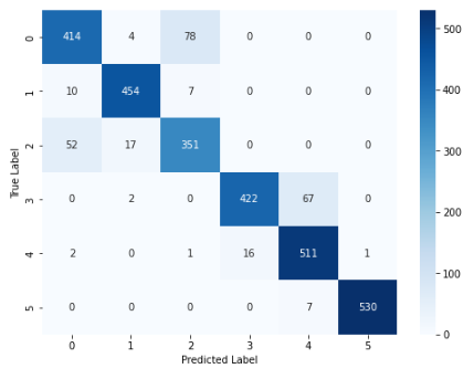
\includegraphics[width=0.9\linewidth,height=0.35\textheight]{figure/ysa_confmat} 

}

\caption{Yapay Sinir Ağları Modeli Karmaşıklık Matrisi}\label{fig:ysaconfmat}
\end{figure}
\begin{figure}

{\centering 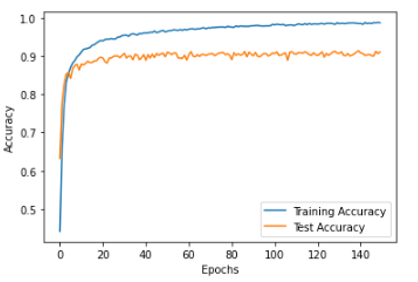
\includegraphics[width=0.6\linewidth,height=0.25\textheight]{figure/ysa_testtrain} 

}

\caption{Jiroskop Sensörü İçin Yapay Sinir Ağları Modelinin Epochs Değerlerine Göre Eğitim ve Test Verilerinin Başarı Performansları}\label{fig:ysatesttrain}
\end{figure}
\hypertarget{ivme-uxf6luxe7er-sensuxf6ruxfcne-ait-deux11fiux15fkenler-ile-modelleme}{%
\section{İvme Ölçer Sensörüne Ait Değişkenler İle Modelleme}\label{ivme-uxf6luxe7er-sensuxf6ruxfcne-ait-deux11fiux15fkenler-ile-modelleme}}

\hypertarget{k-en-yakux131n-komux15fuluk-modeli}{%
\subsection{K-En Yakın Komşuluk Modeli}\label{k-en-yakux131n-komux15fuluk-modeli}}

Bu bölümde ivme ölçer sensöründen elde edilen veriler kullanılmıştır.K-En yakın komşuluk modeli kurulmuş ve çıktıları değerlendirilmiştir.
\ref{tab:nvaracc}.' te belirtilen değişkenler kullanılarak modelleme gerçekleştirilmiştir.

\hypertarget{hiper-parametre-seuxe7imi-4}{%
\subsubsection{Hiper Parametre Seçimi}\label{hiper-parametre-seuxe7imi-4}}

Daha önce belirlenen parametre uzayını ve Scikit-Learn kütüphanesinde bulunan GridSearchCV algoritması ile en yüksek doğruluk oranı yakalanana kadar çalışması sağlanmıştır.
K-En yakın komşuluk modeli için en yüksek doğruluk oranı aşağıdaki parametreler ile bulunmuştur;
\begin{itemize}
\tightlist
\item
  metric: manhattan
\item
  n\_neighbors: 9
\item
  weights: distance
\end{itemize}
\hypertarget{en-iyi-model-5}{%
\subsubsection{En İyi Model}\label{en-iyi-model-5}}

Bulunan parametrelerle kurulan modelin sınıflandırma metrikleri aşağıdaki gibidir.
\begin{longtable}[]{@{}lllll@{}}
\caption{\label{tab:iknn} İvmeölçer Sensöründen elde edilen değişkenler ile kurulan k en yakın komşular algoritmasının başarı sonuçları}\tabularnewline
\toprule()
& precision & recall & F1-score & support \\
\midrule()
\endfirsthead
\toprule()
& precision & recall & F1-score & support \\
\midrule()
\endhead
0 & 0.89 & 0.85 & 0.87 & 496 \\
1 & 0.89 & 0.94 & 0.92 & 471 \\
2 & 0.81 & 0.81 & 0.81 & 420 \\
3 & 0.97 & 0.88 & 0.92 & 491 \\
4 & 0.90 & 0.97 & 0.93 & 531 \\
5 & 1.00 & 1.00 & 1.00 & 537 \\
Accuracy & & & 0.91 & 2946 \\
macro avg & 0.91 & 0.91 & 0.91 & 2946 \\
weighted avg & 0.91 & 0.91 & 0.91 & 2946 \\
\bottomrule()
\end{longtable}
\begin{figure}

{\centering 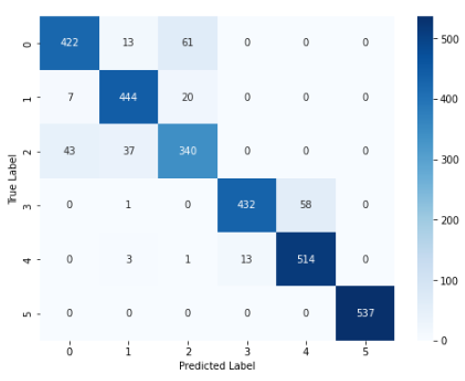
\includegraphics[width=0.9\linewidth,height=0.35\textheight]{figure/iknn_confmat} 

}

\caption{K-NN Modeli Karmaşıklık Matrisi}\label{fig:iknnconfmat}
\end{figure}
\begin{figure}

{\centering 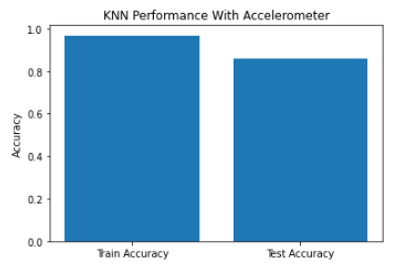
\includegraphics[width=0.6\linewidth,height=0.25\textheight]{figure/iknn_testtrain} 

}

\caption{K-NN Modelinin Eğitim ve Test Verilerinin Başarı Performansları}\label{fig:iknntesttrain}
\end{figure}
\hypertarget{rassal-ormanlar-modeli-1}{%
\subsection{Rassal Ormanlar Modeli}\label{rassal-ormanlar-modeli-1}}

Bu bölümde ivme ölçer sensöründen elde edilen veriler kullanılmıştır.Rassal ormanlar modeli kurulmuş ve çıktıları değerlendirilmiştir.
\ref{tab:nvaracc}.' te belirtilen değişkenler kullanılarak modelleme işlemi gerçekleştirilmiştir.

\hypertarget{hiper-parametre-seuxe7imi-5}{%
\subsubsection{Hiper Parametre Seçimi}\label{hiper-parametre-seuxe7imi-5}}

Daha önce belirlenen parametre uzayını ve Scikit-Learn kütüphanesinde bulunan GridSearchCV algoritması ile en yüksek doğruluk oranı yakalanana kadar çalışması sağlanmıştır.
\begin{itemize}
\tightlist
\item
  max\_depth: 20
\item
  min\_samples\_leaf: 4
\item
  min\_samples\_split: 10
\item
  n\_estimators: 500
\end{itemize}
\hypertarget{en-iyi-model-6}{%
\subsubsection{En İyi Model}\label{en-iyi-model-6}}

Bulunan parametrelerle kurulan modelin sınıflandırma metrikleri aşağıdaki gibidir.
\begin{longtable}[]{@{}lllll@{}}
\caption{\label{tab:irf} İvmeölçer Sensöründen elde edilen değişkenler ile kurulan rassal ormanlar modelinin başarı sonuçları}\tabularnewline
\toprule()
& precision & recall & F1-score & support \\
\midrule()
\endfirsthead
\toprule()
& precision & recall & F1-score & support \\
\midrule()
\endhead
0 & 0.85 & 0.96 & 0.90 & 496 \\
1 & 0.88 & 0.86 & 0.87 & 471 \\
2 & 0.95 & 0.94 & 0.89 & 420 \\
3 & 0.81 & 0.81 & 0.81 & 491 \\
4 & 0.82 & 0.83 & 0.83 & 531 \\
5 & 1.00 & 1.00 & 1.00 & 537 \\
Accuracy & & & 0.88 & 2946 \\
macro avg & 0.89 & 0.88 & 0.88 & 2946 \\
weighted avg & 0.89 & 0.88 & 0.88 & 2946 \\
\bottomrule()
\end{longtable}
\begin{figure}

{\centering 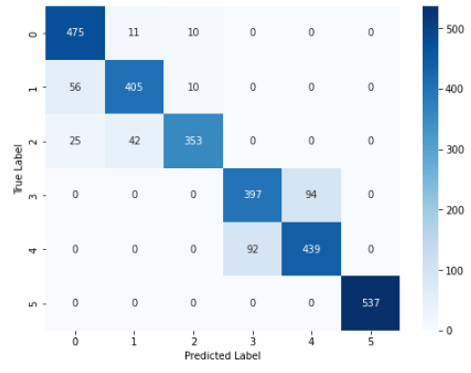
\includegraphics[width=0.9\linewidth,height=0.35\textheight]{figure/irandom_forest_confmat} 

}

\caption{Rassal Ormanlar Modeli Karmaşıklık Matrisi}\label{fig:irandomforestconfmat}
\end{figure}
\begin{figure}

{\centering 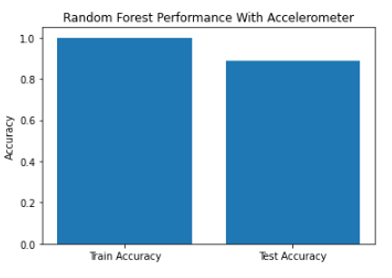
\includegraphics[width=0.6\linewidth,height=0.25\textheight]{figure/irandom_forest_testtrain} 

}

\caption{Rassal Ormanlar Modelinin Eğitim ve Test Verilerinin Başarı Performansları}\label{fig:irandomforesttesttrain}
\end{figure}
\hypertarget{extreme-gradient-boosting-xgboost-1}{%
\subsection{eXtreme Gradient Boosting (XGBoost)}\label{extreme-gradient-boosting-xgboost-1}}

Bu bölümde ivme ölçer sensöründen elde edilen veriler kullanılmıştır.XGBoost modeli kurulmuş ve çıktıları değerlendirilmiştir.
\ref{tab:nvaracc}.' te belirtilen değişkenler kullanılarak modelleme işlemi gerçekleştirilmiştir.

\hypertarget{hiper-parametre-seuxe7imi-6}{%
\subsubsection{Hiper Parametre Seçimi}\label{hiper-parametre-seuxe7imi-6}}

Daha önce belirlenen parametre uzayını ve Scikit-Learn kütüphanesinde bulunan GridSearchCV algoritması ile en yüksek doğruluk oranı yakalanana kadar çalışması sağlanmıştır.
\begin{itemize}
\tightlist
\item
  max\_depth: 3
\item
  learning\_rate: 0.01
\item
  n\_estimators: 100
\end{itemize}
\hypertarget{en-iyi-model-7}{%
\subsubsection{En İyi Model}\label{en-iyi-model-7}}

Bulunan parametrelerle kurulan modelin sınıflandırma metrikleri aşağıdaki gibidir.
\begin{longtable}[]{@{}lllll@{}}
\caption{\label{tab:ixgboost} İvmeölçer Sensöründen elde edilen değişkenler ile kurulan xgboost modelinin başarı sonuçları}\tabularnewline
\toprule()
& precision & recall & F1-score & support \\
\midrule()
\endfirsthead
\toprule()
& precision & recall & F1-score & support \\
\midrule()
\endhead
0 & 0.88 & 0.95 & 0.91 & 496 \\
1 & 0.87 & 0.89 & 0.88 & 471 \\
2 & 0.98 & 0.89 & 0.93 & 420 \\
3 & 0.82 & 0.80 & 0.81 & 491 \\
4 & 0.82 & 0.83 & 0.83 & 531 \\
5 & 1.00 & 1.00 & 1.00 & 537 \\
Accuracy & & & 0.89 & 2946 \\
macro avg & 0.90 & 0.89 & 0.89 & 2946 \\
weighted avg & 0.89 & 0.89 & 0.89 & 2946 \\
\bottomrule()
\end{longtable}
\begin{figure}

{\centering 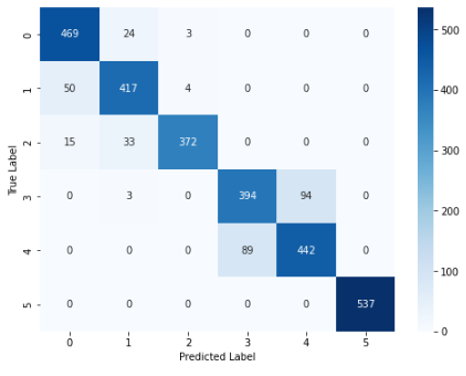
\includegraphics[width=0.9\linewidth,height=0.35\textheight]{figure/ixgboost_confmat} 

}

\caption{Xgboost modeli Karmaşıklık Matrisi}\label{fig:ixgboostconfmat}
\end{figure}
\begin{figure}

{\centering 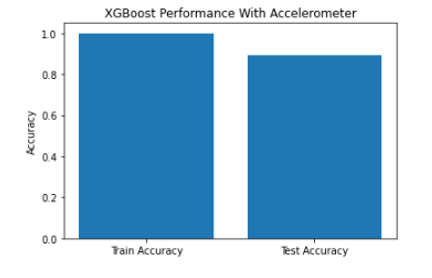
\includegraphics[width=0.6\linewidth,height=0.25\textheight]{figure/ixgboost_testtrain} 

}

\caption{Xgboost Modelinin Eğitim ve Test Verilerinin Başarı Performansları}\label{fig:ixgboosttesttrain}
\end{figure}
\hypertarget{destek-vektuxf6r-makinesi-2}{%
\subsection{Destek Vektör Makinesi}\label{destek-vektuxf6r-makinesi-2}}

Bu bölümde ivme ölçer sensöründen elde edilen veriler kullanılmıştır.Destek Vektör Makinesi (SVM) modeli kurulmuş ve çıktıları değerlendirilmiştir
\ref{tab:nvaracc}.' te belirtilen değişkenler kullanılarak modelleme işlemi gerçekleştirilmiştir.

\hypertarget{hiper-parametre-seuxe7imi-7}{%
\subsubsection{Hiper Parametre Seçimi}\label{hiper-parametre-seuxe7imi-7}}

Daha önce belirlenen parametre uzayını ve Scikit-Learn kütüphanesinde bulunan GridSearchCV algoritması ile en yüksek doğruluk oranı yakalanana kadar çalışması sağlanmıştır.
\begin{itemize}
\tightlist
\item
  C: 0.1
\item
  gamma: 0.01
\item
  kernel: linear
\end{itemize}
\hypertarget{en-iyi-model-8}{%
\subsubsection{En İyi Model}\label{en-iyi-model-8}}

Bulunan parametrelerle kurulan modelin sınıflandırma metrikleri aşağıdaki gibidir.
\begin{longtable}[]{@{}lllll@{}}
\caption{\label{tab:isvm} İvmeölçer Sensöründen elde edilen değişkenler ile kurulan destek vektör makinası algoritmasının başarı sonuçları}\tabularnewline
\toprule()
& precision & recall & F1-score & support \\
\midrule()
\endfirsthead
\toprule()
& precision & recall & F1-score & support \\
\midrule()
\endhead
0 & 0.89 & 0.96 & 0.92 & 496 \\
1 & 0.90 & 0.90 & 0.90 & 471 \\
2 & 0.98 & 0.90 & 0.94 & 420 \\
3 & 0.86 & 0.77 & 0.81 & 491 \\
4 & 0.81 & 0.88 & 0.84 & 531 \\
5 & 1.00 & 1.00 & 1.00 & 537 \\
Accuracy & & & 0.90 & 2946 \\
macro avg & 0.91 & 0.90 & 0.90 & 2946 \\
weighted avg & 0.91 & 0.90 & 0.90 & 2946 \\
\bottomrule()
\end{longtable}
\begin{figure}

{\centering 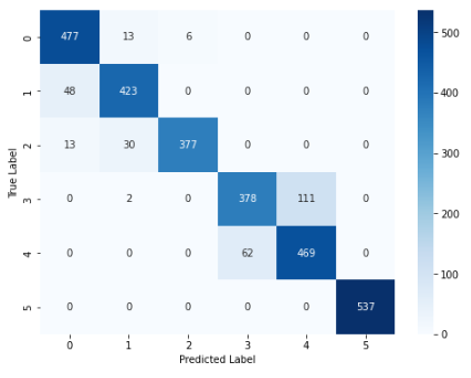
\includegraphics[width=0.9\linewidth,height=0.35\textheight]{figure/isvm_confmat} 

}

\caption{Destek Vektör Makinesi Modeli Karmaşıklık Matrisi}\label{fig:isvmconfmat}
\end{figure}
\begin{figure}

{\centering 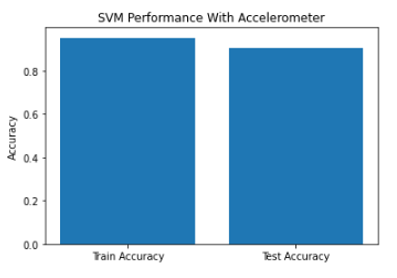
\includegraphics[width=0.6\linewidth,height=0.25\textheight]{figure/isvm_testtrain} 

}

\caption{Destek Vektör Modelinin Eğitim ve Test Verilerinin Başarı Performansları}\label{fig:isvmtesttrain}
\end{figure}
\hypertarget{yapay-sinir-aux11flarux131-neural-networks-1}{%
\subsection{Yapay Sinir Ağları (Neural Networks)}\label{yapay-sinir-aux11flarux131-neural-networks-1}}

Bu bölümde ivme ölçer sensörü üzerinde yapay sinir ağları modeli kullanılmış ve çıktıları değerlendirilmiştir.Tensorflow ve Keras kütüphanelerindeki Sequential() fonksiyonu kullanılmıştır.

\hypertarget{kullanux131lan-katmanlar-1}{%
\subsubsection{Kullanılan Katmanlar}\label{kullanux131lan-katmanlar-1}}

İlk katman, tamamen bağlı (Dense) katmandır. Bu katman 64 nörona sahiptir ve girdi boyutu, train veri kümesinin özellik sayısına eşittir. kernel\_initializer parametresi ``normal'' olarak ayarlanmıştır, yani rastgele normal bir dağılım kullanılarak başlangıç ağırlıkları oluşturulacaktır. Bu katmanın aktivasyon fonksiyonu ``sigmoid'' olarak ayarlanmıştır.
İkinci katman, bir Dropout katmanıdır. Dropout, ağdaki aşırı uyumu azaltmak için kullanılan bir düzenleme tekniğidir. Bu katmanın Dropout oranı \%20 olarak ayarlanmıştır.
Üçüncü ve son katman, yine bir tamamen bağlı (Dense) katmandır. Bu katman 6 nörona sahiptir ve softmax aktivasyon fonksiyonu kullanılarak çoklu sınıflandırma işlemi gerçekleştirilir. kernel\_initializer parametresi ``normal'' olarak ayarlanmıştır.
Modelin derlenmesi, ``adam'' optimizasyon algoritması kullanılarak gerçekleştirilir. Kayıp fonksiyonu ``sparse\_categorical\_crossentropy'' olarak ayarlanmıştır, çünkü etiketler doğrudan kategorik olarak kodlanmamıştır. Ölçülen metrik, doğruluk (accuracy) olarak ayarlanmıştır.
\ref{tab:nvaracc}.' te belirtilen değişkenler kullanılarak modelleme işlemi gerçekleştirilmiştir.

\hypertarget{en-iyi-model-9}{%
\subsubsection{En iyi Model}\label{en-iyi-model-9}}

Kullanılan parametrelerle ve belirtilen epochs değeri ile kurulan modelin sınıflandırma metrikleri aşağıdaki gibidir.
\begin{longtable}[]{@{}lllll@{}}
\caption{\label{tab:iysa} İvmeölçer Sensöründen elde edilen değişkenler ile kurulan yapay sinir ağları modelinin başarı sonuçları}\tabularnewline
\toprule()
& precision & recall & F1-score & support \\
\midrule()
\endfirsthead
\toprule()
& precision & recall & F1-score & support \\
\midrule()
\endhead
0 & 0.89 & 0.98 & 0.93 & 496 \\
1 & 0.95 & 0.87 & 0.91 & 471 \\
2 & 0.98 & 0.95 & 0.97 & 420 \\
3 & 0.85 & 0.81 & 0.83 & 491 \\
4 & 0.82 & 0.86 & 0.84 & 531 \\
5 & 1.00 & 0.97 & 0.99 & 537 \\
Accuracy & & & 0.91 & 2946 \\
macro avg & 0.91 & 0.91 & 0.91 & 2946 \\
weighted avg & 0.91 & 0.91 & 0.91 & 2946 \\
\bottomrule()
\end{longtable}
\begin{figure}

{\centering 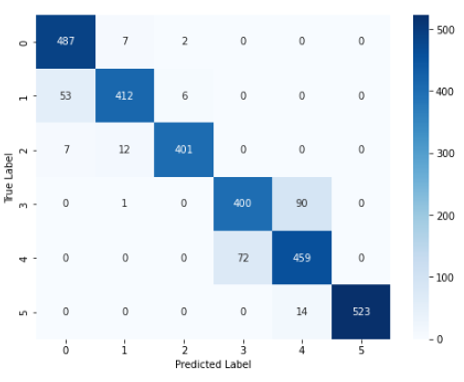
\includegraphics[width=0.9\linewidth,height=0.35\textheight]{figure/iysa_confmat} 

}

\caption{Yapay Sinir Ağları Modeli Karmaşıklık Matrisi}\label{fig:iysaconfmat}
\end{figure}
\begin{figure}

{\centering 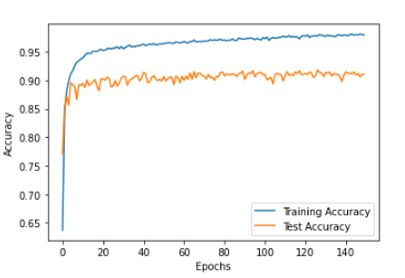
\includegraphics[width=0.6\linewidth,height=0.25\textheight]{figure/iysa_testtrain} 

}

\caption{İvme Ölçer Sensörü İçin Yapay Sinir Ağları Modelinin Epochs Değerlerine Göre Eğitim ve Test Verilerinin Başarı Performansları}\label{fig:iysatesttrain}
\end{figure}
\hypertarget{jiroskop-ve-ivme-uxf6luxe7er-sensuxf6rlerine-ait-deux11fiux15fkenler-ile-modelleme}{%
\section{Jiroskop ve İvme Ölçer Sensörlerine Ait Değişkenler İle Modelleme}\label{jiroskop-ve-ivme-uxf6luxe7er-sensuxf6rlerine-ait-deux11fiux15fkenler-ile-modelleme}}

\hypertarget{k-en-yakux131n-komux15fuluk-modeli-1}{%
\subsection{K-En Yakın Komşuluk Modeli}\label{k-en-yakux131n-komux15fuluk-modeli-1}}

Bu bölümde jiroskop ve ivme ölçer sensörlerinden elde edilen veriler kullanılmıştır.K-En yakın komşuluk modeli kurulmuş ve çıktıları değerlendirilmiştir.
\ref{tab:nvar}.' te belirtilen değişkenler kullanılarak modelleme gerçekleştirilmiştir.

\hypertarget{hiper-parametre-seuxe7imi-8}{%
\subsubsection{Hiper Parametre Seçimi}\label{hiper-parametre-seuxe7imi-8}}

Daha önce belirlenen parametre uzayını ve Scikit-Learn kütüphanesinde bulunan GridSearchCV algoritması ile en yüksek doğruluk oranı yakalanana kadar çalışması sağlanmıştır.
K-En yakın komşuluk modeli için en yüksek doğruluk oranı aşağıdaki parametreler ile bulunmuştur;
\begin{itemize}
\tightlist
\item
  `metric': `manhattan'
\item
  `n\_neighbors': 9
\item
  `weights': `distance'
\end{itemize}
\hypertarget{en-iyi-model-10}{%
\subsubsection{En İyi Model}\label{en-iyi-model-10}}

Bulunan parametrelerle kurulan modelin sınıflandırma metrikleri aşağıdaki gibidir.
\begin{longtable}[]{@{}lllll@{}}
\caption{\label{tab:jiknn} Jiroskop ve İvmeölçer Sensörlerinden elde edilen değişkenler ile kurulan k en yakın komşular modelinin başarı sonuçları}\tabularnewline
\toprule()
& precision & recall & F1-score & support \\
\midrule()
\endfirsthead
\toprule()
& precision & recall & F1-score & support \\
\midrule()
\endhead
0 & 0.87 & 0.98 & 0.92 & 496 \\
1 & 0.88 & 0.92 & 0.90 & 471 \\
2 & 0.98 & 0.78 & 0.87 & 420 \\
3 & 0.96 & 0.82 & 0.89 & 491 \\
4 & 0.86 & 0.97 & 0.91 & 531 \\
5 & 1.00 & 1.00 & 1.00 & 537 \\
Accuracy & & & 0.92 & 2946 \\
macro avg & 0.92 & 0.91 & 0.91 & 2946 \\
weighted avg & 0.92 & 0.92 & 0.92 & 2946 \\
\bottomrule()
\end{longtable}
\begin{figure}

{\centering 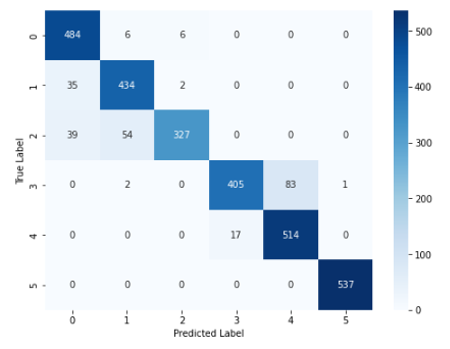
\includegraphics[width=0.9\linewidth,height=0.35\textheight]{figure/jiknn_confmat} 

}

\caption{K-NN Modeli Karmaşıklık Matrisi}\label{fig:jiknnconfmat}
\end{figure}
\begin{figure}

{\centering 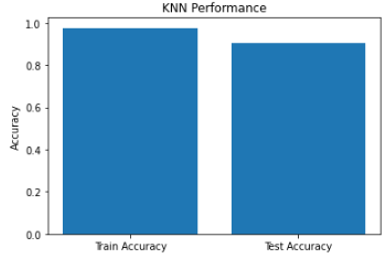
\includegraphics[width=0.6\linewidth,height=0.25\textheight]{figure/jiknn_testtrain} 

}

\caption{K-NN Modelinin Eğitim ve Test Verilerinin Başarı Performansları}\label{fig:jiknntesttrain}
\end{figure}
\hypertarget{rassal-ormanlar-modeli-2}{%
\subsection{Rassal Ormanlar Modeli}\label{rassal-ormanlar-modeli-2}}

Bu bölümde jiroskop ve ivme ölçer sensörlerinden elde edilen veriler kullanılmıştır.Rassal ormanlar modeli kurulmuş ve çıktıları değerlendirilmiştir. \ref{tab:nvar}.' te belirtilen değişkenler kullanılarak modelleme işlemi gerçekleştirilmiştir.

\hypertarget{hiper-parametre-seuxe7imi-9}{%
\subsubsection{Hiper Parametre Seçimi}\label{hiper-parametre-seuxe7imi-9}}

Daha önce belirlenen parametre uzayını ve Scikit-Learn kütüphanesinde bulunan GridSearchCV algoritması ile en yüksek doğruluk oranı yakalanana kadar çalışması sağlanmıştır.
\begin{itemize}
\tightlist
\item
  max\_depth: 20
\item
  min\_samples\_leaf: 4
\item
  min\_samples\_split: 10
\item
  n\_estimators: 500
\end{itemize}
\hypertarget{en-iyi-model-11}{%
\subsubsection{En İyi Model}\label{en-iyi-model-11}}

Bulunan parametrelerle kurulan modelin sınıflandırma metrikleri aşağıdaki gibidir.
\begin{longtable}[]{@{}lllll@{}}
\caption{\label{tab:jirf} Jiroskop ve İvmeölçer Sensörlerinden elde değişkenler ile kurulan rassal ormanlar modelinin başarı sonuçları}\tabularnewline
\toprule()
& precision & recall & F1-score & support \\
\midrule()
\endfirsthead
\toprule()
& precision & recall & F1-score & support \\
\midrule()
\endhead
0 & 0.90 & 0.97 & 0.93 & 496 \\
1 & 0.89 & 0.92 & 0.91 & 471 \\
2 & 0.96 & 0.84 & 0.89 & 420 \\
3 & 0.91 & 0.88 & 0.90 & 491 \\
4 & 0.90 & 0.92 & 0.91 & 531 \\
5 & 1.00 & 1.00 & 1.00 & 537 \\
Accuracy & & & 0.93 & 2946 \\
macro avg & 0.93 & 0.92 & 0.92 & 2946 \\
weighted avg & 0.93 & 0.93 & 0.93 & 2946 \\
\bottomrule()
\end{longtable}
\begin{figure}

{\centering 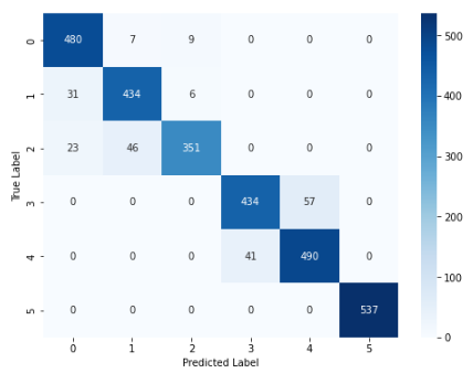
\includegraphics[width=0.9\linewidth,height=0.35\textheight]{figure/ji_random_forest_confmat} 

}

\caption{Rassal Ormanlar Modeli Karmaşıklık Matrisi}\label{fig:jirandomforestconfmat}
\end{figure}
\begin{figure}

{\centering 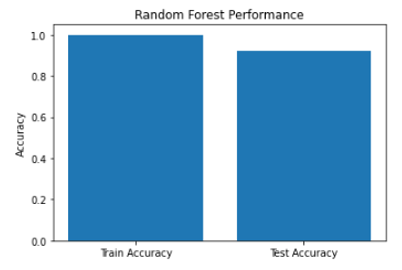
\includegraphics[width=0.6\linewidth,height=0.25\textheight]{figure/ji_random_forest_testtrain} 

}

\caption{Rassal Ormanlar Modelinin Eğitim ve Test Verilerinin Başarı Performansları}\label{fig:jirandomforesttesttrain}
\end{figure}
\hypertarget{extreme-gradient-boosting-xgboost-2}{%
\subsection{eXtreme Gradient Boosting (XGBoost)}\label{extreme-gradient-boosting-xgboost-2}}

Bu bölümde jiroskop ve ivme ölçer sensörlerinden elde edilen veriler kullanılmıştır.XGBoost modeli kurulmuş ve çıktıları değerlendirilmiştir. \ref{tab:nvar}.' te belirtilen değişkenler kullanılarak modelleme işlemi gerçekleştirilmiştir.

\hypertarget{hiper-parametre-seuxe7imi-10}{%
\subsubsection{Hiper Parametre Seçimi}\label{hiper-parametre-seuxe7imi-10}}

Daha önce belirlenen parametre uzayını ve Scikit-Learn kütüphanesinde bulunan GridSearchCV algoritması ile en yüksek doğruluk oranı yakalanana kadar çalışması sağlanmıştır.
\begin{itemize}
\tightlist
\item
  max\_depth: 3
\item
  learning\_rate: 0.01
\item
  n\_estimators: 100
\end{itemize}
\hypertarget{en-iyi-model-12}{%
\subsubsection{En İyi Model}\label{en-iyi-model-12}}

Bulunan parametrelerle kurulan modelin sınıflandırma metrikleri aşağıdaki gibidir.
\begin{longtable}[]{@{}lllll@{}}
\caption{\label{tab:jixgboost} Jiroskop ve İvmeölçer Sensörlerinden elde edilen değişkenler ile kurulan xgboost modelinin başarı sonuçları}\tabularnewline
\toprule()
& precision & recall & F1-score & support \\
\midrule()
\endfirsthead
\toprule()
& precision & recall & F1-score & support \\
\midrule()
\endhead
0 & 0.85 & 0.90 & 0.88 & 496 \\
1 & 0.85 & 0.76 & 0.80 & 471 \\
2 & 0.88 & 0.88 & 0.88 & 420 \\
3 & 0.88 & 0.82 & 0.85 & 491 \\
4 & 0.80 & 0.92 & 0.85 & 531 \\
5 & 1.00 & 0.97 & 0.99 & 537 \\
Accuracy & & & 0.87 & 2946 \\
macro avg & 0.88 & 0.87 & 0.87 & 2946 \\
weighted avg & 0.88 & 0.87 & 0.87 & 2946 \\
\bottomrule()
\end{longtable}
\begin{figure}

{\centering 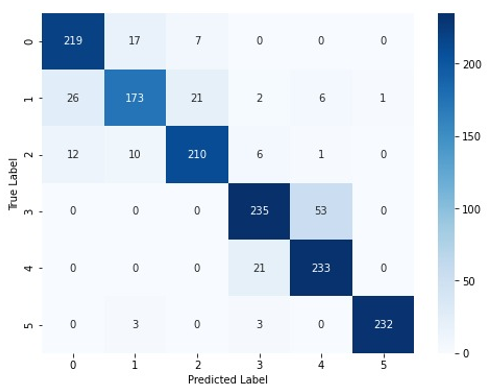
\includegraphics[width=0.9\linewidth,height=0.35\textheight]{figure/jixgboost_confmat} 

}

\caption{XGBoost Modeli Karmaşıklık Matrisi}\label{fig:jixgboostconfmat}
\end{figure}
\begin{figure}

{\centering 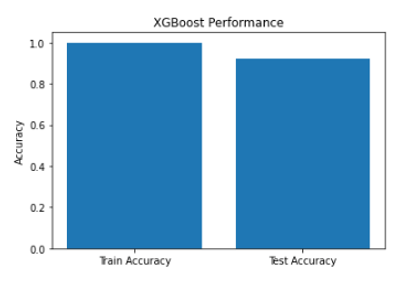
\includegraphics[width=0.6\linewidth,height=0.25\textheight]{figure/jixgboost_testtrain} 

}

\caption{XGBoost Modelinin Eğitim ve Test Verilerinin Başarı Performansları}\label{fig:jixgboosttesttrain}
\end{figure}
\hypertarget{destek-vektuxf6r-makinesi-3}{%
\subsection{Destek Vektör Makinesi}\label{destek-vektuxf6r-makinesi-3}}

Bu bölümde jiroskop ve ivme ölçer sensörlerinden elde edilen veriler kullanılmıştır.Destek Vektör Makinesi (SVM) modeli kurulmuş ve çıktıları değerlendirilmiştir
\ref{tab:nvar}.' te belirtilen değişkenler kullanılarak modelleme işlemi gerçekleştirilmiştir.

\hypertarget{hiper-parametre-seuxe7imi-11}{%
\subsubsection{Hiper Parametre Seçimi}\label{hiper-parametre-seuxe7imi-11}}

Daha önce belirlenen parametre uzayını ve Scikit-Learn kütüphanesinde bulunan GridSearchCV algoritması ile en yüksek doğruluk oranı yakalanana kadar çalışması sağlanmıştır.
\begin{itemize}
\tightlist
\item
  C: 0.1
\item
  gamma: 0.01
\item
  kernel: linear
\end{itemize}
\hypertarget{en-iyi-model-13}{%
\subsubsection{En İyi Model}\label{en-iyi-model-13}}

Bulunan parametrelerle kurulan modelin sınıflandırma metrikleri aşağıdaki gibidir.
\begin{longtable}[]{@{}lllll@{}}
\caption{\label{tab:jisvm} Jiroskop ve İvmeölçer Sensörlerinden elde edilen değişkenler ile kurulan destek vektör makinesi modelinin başarı sonuçları}\tabularnewline
\toprule()
& precision & recall & F1-score & support \\
\midrule()
\endfirsthead
\toprule()
& precision & recall & F1-score & support \\
\midrule()
\endhead
0 & 0.85 & 0.87 & 0.86 & 496 \\
1 & 0.86 & 0.75 & 0.80 & 471 \\
2 & 0.83 & 0.85 & 0.84 & 420 \\
3 & 0.86 & 0.82 & 0.84 & 491 \\
4 & 0.78 & 0.87 & 0.82 & 531 \\
5 & 0.96 & 0.97 & 0.97 & 537 \\
Accuracy & & & 0.85 & 2946 \\
macro avg & 0.86 & 0.85 & 0.85 & 2946 \\
weighted avg & 0.86 & 0.85 & 0.85 & 2946 \\
\bottomrule()
\end{longtable}
\begin{figure}

{\centering 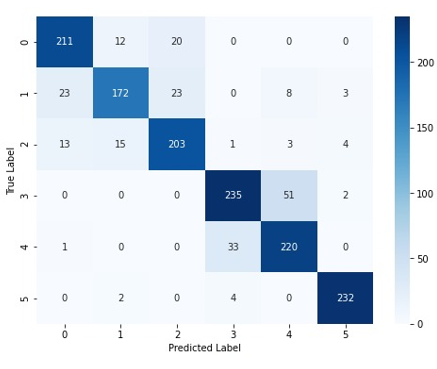
\includegraphics[width=0.9\linewidth,height=0.35\textheight]{figure/jisvm_confmat} 

}

\caption{Destek Vektör Makinesi Modeli Karmaşıklık Matrisi}\label{fig:jisvmconfmat}
\end{figure}
\begin{figure}

{\centering 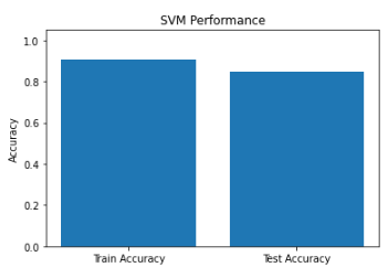
\includegraphics[width=0.6\linewidth,height=0.25\textheight]{figure/jisvm_testtrain} 

}

\caption{Destek Vektör Modelinin Eğitim ve Test Verilerinin Başarı Performansları}\label{fig:jisvmtesttrain}
\end{figure}
\hypertarget{yapay-sinir-aux11flarux131-neural-networks-2}{%
\subsection{Yapay Sinir Ağları (Neural Networks)}\label{yapay-sinir-aux11flarux131-neural-networks-2}}

Bu bölümde jiroskop ve ivme ölçer sensörleri üzerinde yapay sinir ağları modeli kullanılmış ve çıktıları değerlendirilmiştir.Tensorflow ve Keras kütüphanelerindeki Sequential() fonksiyonu kullanılmıştır.

\hypertarget{kullanux131lan-katmanlar-2}{%
\subsubsection{Kullanılan Katmanlar}\label{kullanux131lan-katmanlar-2}}

İlk katman, tamamen bağlı (Dense) katmandır. Bu katman 64 nörona sahiptir ve girdi boyutu, train veri kümesinin özellik sayısına eşittir. kernel\_initializer parametresi ``normal'' olarak ayarlanmıştır, yani rastgele normal bir dağılım kullanılarak başlangıç ağırlıkları oluşturulacaktır. Bu katmanın aktivasyon fonksiyonu ``sigmoid'' olarak ayarlanmıştır.
İkinci katman, bir Dropout katmanıdır. Dropout, ağdaki aşırı uyumu azaltmak için kullanılan bir düzenleme tekniğidir. Bu katmanın Dropout oranı \%20 olarak ayarlanmıştır.
Üçüncü ve son katman, yine bir tamamen bağlı (Dense) katmandır. Bu katman 6 nörona sahiptir ve softmax aktivasyon fonksiyonu kullanılarak çoklu sınıflandırma işlemi gerçekleştirilir. kernel\_initializer parametresi ``normal'' olarak ayarlanmıştır.
Modelin derlenmesi, ``adam'' optimizasyon algoritması kullanılarak gerçekleştirilir. Kayıp fonksiyonu ``sparse\_categorical\_crossentropy'' olarak ayarlanmıştır, çünkü etiketler doğrudan kategorik olarak kodlanmamıştır. Ölçülen metrik, doğruluk (accuracy) olarak ayarlanmıştır.
\ref{tab:nvar}.' te belirtilen değişkenler kullanılarak modelleme işlemi gerçekleştirilmiştir.

\hypertarget{en-iyi-model-14}{%
\subsubsection{En iyi Model}\label{en-iyi-model-14}}

Kullanılan parametrelerle ve belirtilen epochs değeri ile kurulan modelin sınıflandırma metrikleri aşağıdaki gibidir.
\begin{longtable}[]{@{}lllll@{}}
\caption{\label{tab:jiysa} Jiroskop ve İvmeölçer Sensörlerinden elde edilen değişkenler ile kurulan yapay sinir ağları modelinin başarı sonuçları}\tabularnewline
\toprule()
& precision & recall & F1-score & support \\
\midrule()
\endfirsthead
\toprule()
& precision & recall & F1-score & support \\
\midrule()
\endhead
0 & 0.93 & 1.00 & 0.96 & 496 \\
1 & 0.95 & 0.92 & 0.93 & 471 \\
2 & 0.99 & 0.94 & 0.96 & 420 \\
3 & 0.95 & 0.91 & 0.93 & 491 \\
4 & 0.92 & 0.95 & 0.94 & 531 \\
5 & 1.00 & 1.00 & 1.00 & 537 \\
Accuracy & & & 0.95 & 2946 \\
macro avg & 0.96 & 0.95 & 0.95 & 2946 \\
weighted avg & 0.96 & 0.95 & 0.95 & 2946 \\
\bottomrule()
\end{longtable}
\begin{figure}

{\centering 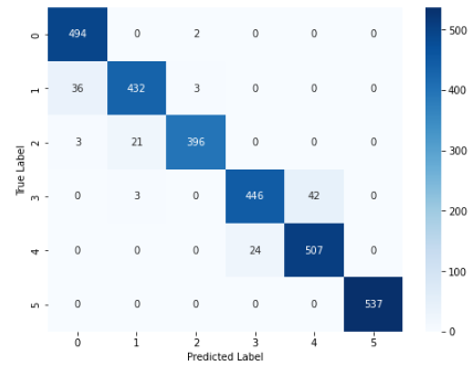
\includegraphics[width=0.6\linewidth,height=0.35\textheight]{figure/jiysa_confmat} 

}

\caption{Yapay Sinir Ağları Modeli Karmaşıklık Matrisi}\label{fig:jiysaconfmat}
\end{figure}
\begin{figure}

{\centering 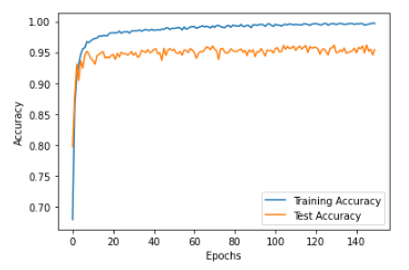
\includegraphics[width=0.6\linewidth,height=0.25\textheight]{figure/jiysa_testtrain} 

}

\caption{Jiroskop ve İvme Ölçer Sensörleri İçin Yapay Sinir Ağları Modelinin Epochs Değerlerine Göre Eğitim ve Test Verilerinin Başarı Performansları}\label{fig:jiysatesttrain}
\end{figure}
\hypertarget{red-labels}{%
\chapter{Sonuç}\label{red-labels}}

Bu çalışmada, insan aktivitelerini tanımak için makine öğrenmesi yöntemleri kullanarak modeller geliştirilmiştir. Farklı modeller arasında karşılaştırma yaparak en iyi sonucu elde etmek için çeşitli deneyler gerçekleştirilmiştir.
Tablo \ref{tab:sonuc}'a göre, sadece jiroskop sensöründen elde edilen değişkenler ile geliştirilen modeller arasında en başarılı sonuç Rassal Ormanlar, Destek Vektör Makinesi ve Yapay Sinir Ağları modelleri ile elde edilmiştir. Sadece ivmeölçer sensöründen elde edilen değişkenler ile geliştirilen modeller arasında en başarılı sonuç K en yakın komşular ve Yapay sinir ağları modelleri ile elde edilmiştir. Her iki sensörle elde edilen değişkenler ile geliştirilen modeler arasında en başarılı sonuç Yapay Sinir Ağları Modeli ile elde edilmiştir
Yapay sinir ağları modeli, karmaşık ilişkileri yakalama yeteneğiyle öne çıkmıştır. Derin öğrenme tabanlı modelin eğitimi için geniş bir veri kümesi kullanılmıştır ve ardından modeli optimize etmek için çeşitli hiperparametre ayarlamaları yapılmıştır. Bu ayarlamaları GridSearchCV algoritması yardımı ile yapılmıştır. Modeli eğitirken, aşırı öğrenmeyi önlemek için Droupout tekniği uygulanmıştır.
Sonuçlar, yapay sinir ağları modelinin, yüksek bir doğruluk oranı ve genel performans ile insan aktivitelerini tanımada diğer modellere göre daha başarılı olduğunu göstermiştir. Bu model, farklı aktiviteler arasında hassas bir şekilde ayrım yapabilmiş ve gerçek zamanlı uygulamalarda kullanıma uygun olduğu düşünülmüştür.
Bu proje, insan aktivitelerini otomatik olarak tanımlayarak sağlık izleme sistemleri, yaşlı bakımı, spor performans analizi ve güvenlik uygulamaları gibi birçok alanda kullanılabilir. Yapay sinir ağları tabanlı modelimizin geliştirilmesi, insan aktivitelerini anlama ve analiz etme konusunda yeni fırsatlar~sunmaktadır.
\begin{longtable}[]{@{}lccl@{}}
\caption{\label{tab:sonuc} Yöntemlere ve Sensörlere göre F1 skorları}\tabularnewline
\toprule()
Yöntemler & Jiroskop & İvmeölçer & Jiroskop ve İvmeölçer \\
\midrule()
\endfirsthead
\toprule()
Yöntemler & Jiroskop & İvmeölçer & Jiroskop ve İvmeölçer \\
\midrule()
\endhead
KNN & 0.82 & 0.91 & 0.91 \\
Rassal Ormanlar & 0.91 & 0.88 & 0.92 \\
XGBoost & 0.89 & 0.89 & 0.87 \\
Destek Vektör Makinesi & 0.91 & 0.90 & 0.85 \\
Yapay Sinir Ağları & 0.91 & 0.91 & 0.95 \\
\bottomrule()
\end{longtable}
\hypertarget{kaynaklar}{%
\chapter*{Kaynaklar}\label{kaynaklar}}
\addcontentsline{toc}{chapter}{Kaynaklar}

\markboth{Kaynaklar}{Kaynaklar}

\hypertarget{refs}{}
\begin{CSLReferences}{1}{0}
\leavevmode\vadjust pre{\hypertarget{ref-augyar2015yapay}{}}%
Ağyar, Z. (2015). Yapay sinir a{ğ}lar{ı}n{ı}n kullan{ı}m alanlar{ı} ve bir uygulama. \emph{M{ü}hendis ve Makine}, \emph{56}(662), 22-23.

\leavevmode\vadjust pre{\hypertarget{ref-anguita2013public}{}}%
Anguita, D., Ghio, A., Oneto, L., Parra, X., Reyes-Ortiz, J. L., ve diğerleri. (2013). A public domain dataset for human activity recognition using smartphones. \emph{Esann} içinde (C. 3, s. 3).

\leavevmode\vadjust pre{\hypertarget{ref-asilkan2009ikinci}{}}%
Asilkan, Ö. ve Irmak, A. G. S. (2009). {İ}kinci el otomobillerin gelecekteki fiyatlarinin yapay sinir a{ğ}lari ile tahmin edilmesi. \emph{S{ü}leyman Demirel {Ü}niversitesi {İ}ktisadi ve {İ}dari Bilimler Fak{ü}ltesi Dergisi}, \emph{14}(2), 375-391.

\leavevmode\vadjust pre{\hypertarget{ref-detienne2003neural}{}}%
Bell, K., Detienne, D. H. ve Joshi, S. A. (2003). Neural networks as statistical tools for business researchers. \emph{Organizational Research Methods}, \emph{6}(2), 236-265.

\leavevmode\vadjust pre{\hypertarget{ref-bengio2013representation}{}}%
Bengio, Y., Courville, A. ve Vincent, P. (2013). Representation learning: A review and new perspectives. \emph{IEEE transactions on pattern analysis and machine intelligence}, \emph{35}(8), 1798-1828.

\leavevmode\vadjust pre{\hypertarget{ref-biau2016random}{}}%
Biau, G. ve Scornet, E. (2016). A random forest guided tour. \emph{Test}, \emph{25}, 197-227.

\leavevmode\vadjust pre{\hypertarget{ref-buduma2017fundamentals}{}}%
Buduma, N. (2017). Fundamentals of Deep Learning, O'Relly Media. Inc.

\leavevmode\vadjust pre{\hypertarget{ref-chen2012sensor}{}}%
Chen, L., Hoey, J., Nugent, C. D., Cook, D. J. ve Yu, Z. (2012). Sensor-based activity recognition. \emph{IEEE Transactions on Systems, Man, and Cybernetics, Part C (Applications and Reviews)}, \emph{42}(6), 790-808.

\leavevmode\vadjust pre{\hypertarget{ref-dandil2020dog}{}}%
Dandıl, E. ve Polattimur, R. (2020). Dog behavior recognition and tracking based on faster R-CNN. \emph{Journal of the Faculty of Engineering and Architecture of Gazi University}, \emph{35}(2), 819-834.

\leavevmode\vadjust pre{\hypertarget{ref-dolgun2009veri}{}}%
Dolgun, M. Ö., Özdemir, T. G. ve Oğuz, D. (2009). Veri madencili{ğ}i{â} nde yap{ı}sal olmayan verinin analizi: Metin ve web madencili{ğ}i. \emph{{İ}statistik{ç}iler Dergisi: {İ}statistik ve Akt{ü}erya}, \emph{2}(2), 48-58.

\leavevmode\vadjust pre{\hypertarget{ref-du2015skeleton}{}}%
Du, Y., Fu, Y. ve Wang, L. (2015). Skeleton based action recognition with convolutional neural network. \emph{2015 3rd IAPR Asian conference on pattern recognition (ACPR)} içinde (ss. 579-583). IEEE.

\leavevmode\vadjust pre{\hypertarget{ref-ecsref2019turkcce}{}}%
Eşref, Y. (2019). T{ü}rk{ç}e Dizi Etiketleme {İ}{ç}in Sinir A{ğ} Modelleri.

\leavevmode\vadjust pre{\hypertarget{ref-fan2013human}{}}%
Fan, L., Wang, Z. ve Wang, H. (2013). Human activity recognition model based on decision tree. \emph{2013 International Conference on Advanced Cloud and Big Data} içinde (ss. 64-68). IEEE.

\leavevmode\vadjust pre{\hypertarget{ref-firat2004aski}{}}%
Fırat, M. ve Güngör, M. (2004). Ask{ı} madde konsantrasyonu ve miktar{ı}n{ı}n yapay sinir a{ğ}lar{ı} ile belirlenmesi. \emph{Teknik Dergi}, \emph{15}(73).

\leavevmode\vadjust pre{\hypertarget{ref-hanbay2020hyperspectral}{}}%
Hanbay, K. (2020). Hyperspectral image classification using convolutional neural network and two-dimensional complex Gabor transform. \emph{Journal of the Faculty of Engineering and Architecture of Gazi University}, \emph{35}(1), 443-456.

\leavevmode\vadjust pre{\hypertarget{ref-icsik2020turkish}{}}%
Isık, G. ve Artuner, H. (2020). Turkish dialect recognition in terms of prosodic by long short-term memory neural networks. \emph{Journal of the Faculty of Engineering and Architecture of Gazi University}, \emph{35}(1).

\leavevmode\vadjust pre{\hypertarget{ref-iskanderov2019akilli}{}}%
Iskanderov, J. ve Güvensan, M. A. (2019). Ak{ı}ll{ı} telefon ve giyilebilir cihazlarla aktivite tan{ı}ma: Klasik yakla{ş}{ı}mlar, yeni {ç}{ö}z{ü}mler. \emph{Pamukkale {Ü}niversitesi M{ü}hendislik Bilimleri Dergisi}, \emph{25}(2), 223-239.

\leavevmode\vadjust pre{\hypertarget{ref-kelle2022mqtt}{}}%
Kelle, A. C. ve Hüseyin, Y. (2022). MQTT Trafi{ğ}inde DoS Sald{ı}r{ı}lar{ı}n{ı}n Makine {Ö}{ğ}renmesi ile S{ı}n{ı}fland{ı}r{ı}lmas{ı} ve Modelin SHAP ile Yorumlanmas{ı}. \emph{Journal of Materials and Mechatronics: A}, \emph{3}(1), 50-62.

\leavevmode\vadjust pre{\hypertarget{ref-khan2008accelerometer}{}}%
Khan, A. M., Lee, Y.-K. ve Kim, T.-S. (2008). Accelerometer signal-based human activity recognition using augmented autoregressive model coefficients and artificial neural nets. \emph{2008 30th Annual International Conference of the IEEE Engineering in Medicine and Biology Society} içinde (ss. 5172-5175). IEEE.

\leavevmode\vadjust pre{\hypertarget{ref-kuncan2019new}{}}%
Kuncan, F. ve Kaya, M., Yılmaz. (2019). New approaches based on local binary patterns for gender identification from sensor signals. \emph{Journal of the Faculty of Engineering and Architecture of Gazi University}, \emph{34}(4), 2173-2185.

\leavevmode\vadjust pre{\hypertarget{ref-kwapisz2011activity}{}}%
Kwapisz, J. R., Weiss, G. M. ve Moore, S. A. (2011). Activity recognition using cell phone accelerometers. \emph{ACM SigKDD Explorations Newsletter}, \emph{12}(2), 74-82.

\leavevmode\vadjust pre{\hypertarget{ref-lantz2019machine}{}}%
Lantz, B. (2019). \emph{Machine learning with R: expert techniques for predictive modeling}. Packt publishing ltd.

\leavevmode\vadjust pre{\hypertarget{ref-lecun1998gradient}{}}%
LeCun, Y., Bottou, L., Bengio, Y. ve Haffner, P. (1998). Gradient-based learning applied to document recognition. \emph{Proceedings of the IEEE}, \emph{86}(11), 2278-2324.

\leavevmode\vadjust pre{\hypertarget{ref-lim2019internet}{}}%
Lim, T. W. (2019). The Internet of Things (IoT). \emph{Industrial Revolution 4.0, Tech Giants, and Digitized Societies} içinde (ss. 33-49). Springer.

\leavevmode\vadjust pre{\hypertarget{ref-maltarollo2013applications}{}}%
Maltarollo, V. G., Honório, K. M. ve Silva, A. B. F. da. (2013). Applications of artificial neural networks in chemical problems. \emph{Artificial neural networks-architectures and applications}, 203-223.

\leavevmode\vadjust pre{\hypertarget{ref-mandic2001recurrent}{}}%
Mandic, D. ve Chambers, J. (2001). \emph{Recurrent neural networks for prediction: learning algorithms, architectures and stability}. Wiley.

\leavevmode\vadjust pre{\hypertarget{ref-metin2021insanin}{}}%
Metin, İ. A. ve Karasulu, B. (2021a). {İ}nsan{ı}n g{ü}nl{ü}k aktivitelerinin yeni bir veri k{ü}mesi: Derin {ö}{ğ}renme tekniklerini kullanarak s{ı}n{ı}fland{ı}rma performans{ı} i{ç}in k{ı}yaslama sonu{ç}lar{ı}. \emph{Gazi {Ü}niversitesi M{ü}hendislik Mimarl{ı}k Fak{ü}ltesi Dergisi}, \emph{36}(2), 759-778.

\leavevmode\vadjust pre{\hypertarget{ref-metin2021novel}{}}%
Metin, İ. A. ve Karasulu, B. (2021b). A novel dataset of human daily activities: Its benchmarking results for classification performance via using deep learning techniques. \emph{Journal of the Faculty of Engineering and Architecture of Gazi University}, \emph{36}(2), 759-777.

\leavevmode\vadjust pre{\hypertarget{ref-metin2019insan}{}}%
Metın, İ. A. ve Karasulu, B. (2019). {İ}nsan aktivitelerinin s{ı}n{ı}fland{ı}r{ı}lmas{ı}nda tekrarlayan sinir a{ğ}{ı} kullanan derin {ö}{ğ}renme tabanl{ı} yakla{ş}{ı}m. \emph{Veri Bilimi}, \emph{2}(2), 1-10.

\leavevmode\vadjust pre{\hypertarget{ref-ozturk2018yapay}{}}%
Öztürk, K. ve Şahin, M. E. (2018). Yapay sinir a{ğ}lar{ı} ve yapay zek{â}'ya genel bir bak{ı}{ş}. \emph{Takvim-i Vekayi}, \emph{6}(2), 25-36.

\leavevmode\vadjust pre{\hypertarget{ref-paul2015effective}{}}%
Paul, P. ve George, T. (2015). An effective approach for human activity recognition on smartphone. \emph{2015 IEEE International Conference on Engineering and Technology (ICETECH)} içinde (ss. 1-3). IEEE.

\leavevmode\vadjust pre{\hypertarget{ref-riboni2011cosar}{}}%
Riboni, D. ve Bettini, C. (2011). COSAR: hybrid reasoning for context-aware activity recognition. \emph{Personal and Ubiquitous Computing}, \emph{15}(3), 271-289.

\leavevmode\vadjust pre{\hypertarget{ref-saugbacs2017akilli}{}}%
Sağbaş, E. A. ve Ballı, S. (2017). Ak{ı}ll{ı} saat alg{ı}lay{ı}c{ı}lar{ı} ile insan hareketlerinin s{ı}n{ı}fland{ı}r{ı}lmas{ı}. \emph{S{ü}leyman Demirel {Ü}niversitesi Fen Bilimleri Enstit{ü}s{ü} Dergisi}, \emph{21}(3), 980-990.

\leavevmode\vadjust pre{\hypertarget{ref-saugbacs2021akilli}{}}%
Sağbaş, E. A., Korukoğlu, S. ve Ballı, S. (2021). AKILLI TELEFON VER{.I}LER{.I} VE MAK{.I}NE {"O}{Ğ}RENMES{.I} Y{"O}NTEMLER{.I} KULLANILARAK STRES TESP{.I}T{.I} {Ç}ALI{Ş}MALARI {"U}ZER{.I}NE B{.I}R L{.I}TERAT{"U}R ARA{Ş}TIRMASI. \emph{M{"u}hendislik Bilimleri ve Tasar{ı}m Dergisi}, \emph{9}(3), 1030-1038.

\leavevmode\vadjust pre{\hypertarget{ref-schuster1997bidirectional}{}}%
Schuster, M. ve Paliwal, K. K. (1997). Bidirectional recurrent neural networks. \emph{IEEE transactions on Signal Processing}, \emph{45}(11), 2673-2681.

\leavevmode\vadjust pre{\hypertarget{ref-tebelskis1995speech}{}}%
Tebelskis, J. M. (1995). \emph{Speech recognition using neural networks}. Carnegie Mellon University.

\leavevmode\vadjust pre{\hypertarget{ref-ustev2013user}{}}%
Ustev, Y. E., Durmaz Incel, O. ve Ersoy, C. (2013). User, device and orientation independent human activity recognition on mobile phones: Challenges and a proposal. \emph{Proceedings of the 2013 ACM conference on Pervasive and ubiquitous computing adjunct publication} içinde (ss. 1427-1436).

\leavevmode\vadjust pre{\hypertarget{ref-yang2008using}{}}%
Yang, J.-Y., Wang, J.-S. ve Chen, Y.-P. (2008). Using acceleration measurements for activity recognition: An effective learning algorithm for constructing neural classifiers. \emph{Pattern recognition letters}, \emph{29}(16), 2213-2220.

\leavevmode\vadjust pre{\hypertarget{ref-yang2016multi}{}}%
Yang, Z., Salakhutdinov, R. ve Cohen, W. (2016). Multi-task cross-lingual sequence tagging from scratch. \emph{arXiv preprint arXiv:1603.06270}.

\leavevmode\vadjust pre{\hypertarget{ref-yangin2019xgboost}{}}%
Yangın, G. (2019). \emph{XGboost ve Karar A{ğ}ac{ı} tabanl{ı} algoritmalar{ı}n diyabet veri setleri {ü}zerine uygulamas{ı}}. (Yayımlanmamış mathesis). Mimar Sinan G{ü}zel Sanatlar {Ü}niversitesi.

\end{CSLReferences}
\setlength{\parindent}{-0.20in}
\setlength{\leftskip}{0.20in}
\setlength{\parskip}{8pt}




\end{document}
